\chapter{Foundations for inference}
\label{foundationsForInference}

Statistical inference is concerned primarily with understanding the quality of parameter estimates. For example, a classic inferential question is, ``How sure are we that the estimated mean, $\bar{x}$, is near the true population mean, $\mu$?'' While the equations and details change depending on the setting, the foundations for inference are the same throughout all of statistics. We introduce these common themes in Sections~\ref{variabilityInEstimates}-\ref{cltSection} by discussing inference about the population mean, $\mu$, and set the stage for other parameters and scenarios in Section~\ref{aFrameworkForInference}. Understanding this chapter will make the rest of this book, and indeed the rest of statistics, seem much more familiar.

\index{data!yrbss|(}

Throughout the next few sections we consider a data set called \data{yrbss}, which represents all 13,583 high school students in the Youth Risk Behavior Surveillance System (YRBSS) from 2013.\footnote{\oiRedirect{textbook-yrbss}{www.cdc.gov/healthyyouth/data/yrbs/data.htm}} Part of this data set is shown in Table~\ref{yrbssDF}, and the variables are described in Table~\ref{yrbssVariables}.

\begin{table}[h]
\centering
\begin{tabular}{rrllrrlrr}
  \hline
ID & age & gender & grade & height & weight & helmet & active & lifting \\ 
  \hline
1 &  14 & female & 9 &  &  & never &   4 &   0 \\ 
  2 &  14 & female & 9 &  &  & never &   2 &   0 \\ 
  3 &  15 & female & 9 & 1.73 & 84.37 & never &   7 &   0 \\ 
  $\vdots$ & $\vdots$ & $\vdots$ & $\vdots$ & $\vdots$ & $\vdots$ & $\vdots$ & $\vdots$ & $\vdots$ \\
  13582 &  17 & female & 12 & 1.60 & 77.11 & sometimes &   5 &  \\ 
  13583 &  17 & female & 12 & 1.57 & 52.16 & did not ride &   5 &  \\ 
  \hline
\end{tabular}
\caption{Five cases from the \data{yrbss} data set. Some observations are blank since there are missing data. For example, the height and weight of students 1 and 2 are missing.\textC{\vspace{-2mm}}}
\label{yrbssDF}
\end{table}
% library(openintro); library(xtable); data(yrbss); xtable(rbind(head(yrbss, 4), tail(yrbss, 2))[, c("age", "gender", "grade", "height", "weight", "helmet_12m", "physically_active_7d", "strength_training_7d")])

\begin{table}[h]
\centering\small
\begin{tabular}{l p{110mm}}
\hline
{\bf age} & {\bf Age of the student.} \\
\hline
\var{gender} & {Sex of the student.} \\
\var{grade} & Grade in high school \\
\var{height} & Height, in meters. There are 3.28 feet in a meter. \\
\var{weight} & Weight, in kilograms (2.2 pounds per kilogram). \\
\var{helmet} & Frequency that the student wore a helmet while biking in the last 12~months. \\
\var{active} & Number of days physically active for 60+ minutes in the last 7 days. \\
\var{lifting} & Number of days of strength training (e.g. lifting weights) in the last 7 days. \\
\hline
\end{tabular}
\caption{Variables and their descriptions for the \data{yrbss} data set.}
\label{yrbssVariables}
\end{table}

\index{data!yrbss\_samp|(}

We're going to consider the population of high school students who participated in the 2013 YRBSS. We took a simple random sample of this population, which is represented in Table~\ref{yrbssSampDF}.\footnote{About 10\% of high schoolers for each variable chose not to answer the question, we used multiple regression (see Chapter~\ref{multipleAndLogisticRegression}) to predict what those responses would have been. For simplicity, we will assume that these predicted values are exactly the truth.} We will use this sample, which we refer to as the \data{yrbss\_samp} data set, to draw conclusions about the population of YRBSS participants. This is the practice of statistical inference in the broadest sense. Two histograms summarizing the \var{height}, \var{weight}, \var{active}, and \var{lifting} variables from \data{yrbss\_samp} data set are shown in Figure~\ref{yrbssSampHistograms}.

\begin{table}
\centering
\begin{tabular}{rrllrrlrr}
  \hline
ID & age & gender & grade & height & weight & helmet & active & lifting \\ 
  \hline
5653 &  16 & female & 11 & 1.50 & 52.62 & never &   0 &   0 \\ 
  9437 &  17 & male & 11 & 1.78 & 74.84 & rarely &   7 &   5 \\ 
  2021 &  17 & male & 11 & 1.75 & 106.60 & never &   7 &   0 \\ 
  $\vdots$ & $\vdots$ & $\vdots$ & $\vdots$ & $\vdots$ & $\vdots$ & $\vdots$ & $\vdots$ & $\vdots$ \\
  2325 &  14 & male & 9 & 1.70 & 55.79 & never &   1 &   0 \\ 
   \hline
\end{tabular}
\caption{Four observations for the \data{yrbss\_samp} data set, which represents a simple random sample of 100 high schoolers from the 2013 YRBSS.}
\label{yrbssSampDF}
% library(openintro); library(xtable); data(yrbss); xtable(rbind(head(yrbss.samp, 3), tail(yrbss.samp, 1))[, c("age", "gender", "grade", "height", "weight", "helmet_12m", "physically_active_7d", "strength_training_7d")])
%library(openintro); library(xtable); data(yrbss); data(yrbss.samp); xtable(yrbss.amp[c(1,2,3,100),])
\end{table}

% WARNING: This figure is referenced in Section 4.2
\begin{figure}
\centering
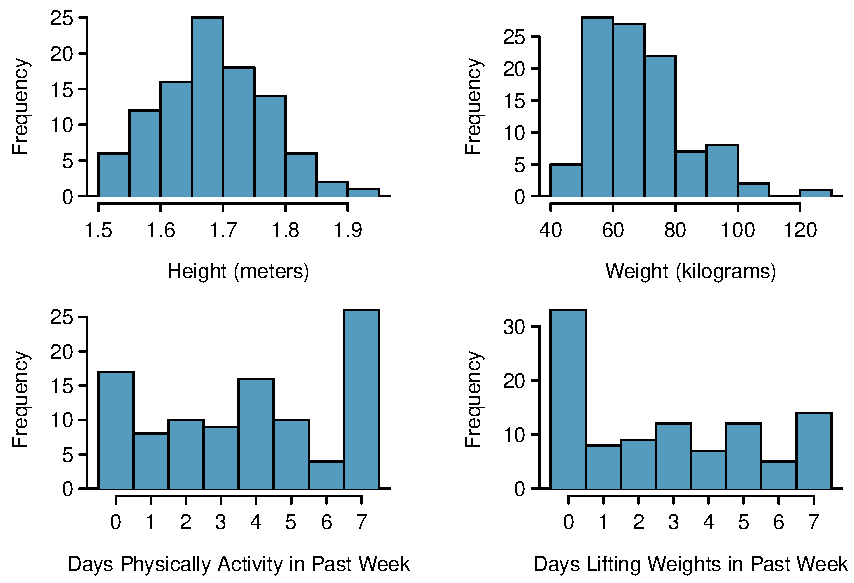
\includegraphics[width=0.8\textwidth]{ch_inference_foundations/figures/yrbssSampHistograms/yrbssSampHistograms} 
\caption{Histograms of \var{height}, \var{weight}, \var{activity}, and \var{lifting} for the sample YRBSS data. The \var{height} distribution is approximately symmetric, \var{weight} is moderately skewed to the right, \var{activity} is bimodal or multimodal (with unclear skew), and \var{lifting} is strongly right skewed.\index{skew!example: moderate}\index{skew!example: strong}}
\label{yrbssSampHistograms}
\end{figure}


%__________________
\section[Variability in estimates]{Variability in estimates \sectionvideohref{youtube-DNIauUrRIEM&list=PLkIselvEzpM7Pjo94m1e7J5jkIZkbQAl4}}
\label{variabilityInEstimates}

\index{point estimate|(}

We would like to estimate four features of the high schoolers in YRBSS using the sample.
\begin{itemize}
\setlength{\itemsep}{0mm}
\item[(1)] What is the average height of the YRBSS high schoolers?
\item[(2)] What is the average weight of the YRBSS high schoolers?
\item[(3)] On average, how many days per week are YRBSS high schoolers physically active?
\item[(4)] On average, how many days per week do YRBSS high schoolers do weight training?
\end{itemize}
While we focus on the mean in this chapter, questions regarding variation are often just as important in practice. For instance, if students are either very active or almost entirely inactive (the distribution is bimodal), we might try different strategies to promote a healthy lifestyle among students than if all high schoolers were already somewhat active.

% We will use $x_1, ..., x_{100}$ to represent the heights for each high schooler in our sample, and $y_1, ..., y_{100}$ will represent their weights.

\subsection{Point estimates}
\label{pointEstimates}

\index{point estimate!single mean|(}

We want to estimate the \term{population mean} based on the sample. The most intuitive way to go about doing this is to simply take the \term{sample mean}. That is, to estimate the average height of all YRBSS students, take the average height for the sample:
\begin{eqnarray*}
\bar{x}_{height} = \frac{1.50 + 1.78 + \dots + 1.70}{100} = 1.697
\end{eqnarray*}
%library(openintro); data(yrbss.samp); mean(yrbss.samp$height); yrbss.samp$height
The sample mean $\bar{x} = 1.697$ meters (5 feet, 6.8 inches) is called a \term{point estimate} of the population mean: if we can only choose one value to estimate the population mean, this is our best guess. Suppose we take a new sample of 100 people and recompute the mean; we will probably not get the exact same answer that we got using the \data{yrbss\_samp} data set. Estimates generally vary from one sample to another, and this \term{sampling variation} suggests our estimate may be close, but it will not be exactly equal to the parameter.

We can also estimate the average weight of YRBSS respondents by examining the sample mean of \var{weight} (in kg), and average number of days physically active in a~week:
\begin{align*}
\bar{x}_{weight} &= \frac{52.6 + 74.8 + \dots + 55.8}{100} = 68.89
&\bar{x}_{active} &= \frac{0 + 7 + \dots + 1}{100} = 3.75
\end{align*}
%library(openintro); data(yrbss.samp); d <- yrbss.samp$weight; mean(d); d
%library(openintro); data(yrbss.samp); d <- yrbss.samp$physically_active_7d; mean(d); d
The average weight is 68.89 kilograms, which is about 151.6 pounds.

What about generating point estimates of other \term{population parameters}, such as the population median or population standard deviation? Once again we might estimate parameters based on sample statistics, as shown in Table~\ref{ptEstimatesYrbssActive}. For example, the population standard deviation of \var{active} using the sample standard deviation, 2.56~days.

\begin{table}[h]
\centering
\begin{tabular}{ l rr}
\hline
\var{active}	& estimate & parameter  \\
\hline
mean		& 3.75 & 3.90 \\
median		& 4.00 & 4.00 \\
st. dev.		& 2.556 & 2.564 \\
\hline
\end{tabular}
\caption{Point estimates and parameter values for the \var{active} variable. The parameters were obtained by computing the mean, median, and SD for all YRBSS respondents.}
\label{ptEstimatesYrbssActive}
\end{table}
%library(openintro); library(xtable); data(yrbss); data(yrbss.samp); d <- yrbss.samp$physically_active_7d; mean(d); median(d); sd(d); d <- yrbss$physically_active_7d; mean(d, na.rm = TRUE); median(d, na.rm = TRUE); sd(d, na.rm = TRUE)


\begin{exercise} \label{peOfDiffActiveBetweenGender}
Suppose we want to estimate the difference in days active for men and women. If $\bar{x}_{men} = 4.3$ and $\bar{x}_{women} = 3.2$, then what would be a good point estimate for the population difference?\footnote{We could take the difference of the two sample means: $4.3 - 3.2 = 1.1$. Men are physically active about 1.1 days per week more than women on average in YRBSS.}
\end{exercise}
%library(openintro); library(xtable); data(yrbss); data(yrbss.samp); (x <- by(yrbss.samp$physically_active_7d, yrbss.samp$gender, mean)); diff(x)

\begin{exercise}
If you had to provide a point estimate of the population IQR for the heights of participants, how might you make such an estimate using a sample?\footnote{To obtain a point estimate of the height for the full set of YRBSS students, we could take the IQR of the sample.}

\index{point estimate!single mean|)}

\end{exercise}

\subsection{Point estimates are not exact}

Estimates are usually not exactly equal to the truth, but they get better as more data become available. We can see this by plotting a running mean from \data{yrbss\_samp}. A \term{running mean} is a sequence of means, where each mean uses one more observation in its calculation than the mean directly before it in the sequence. For example, the second mean in the sequence is the average of the first two observations and the third in the sequence is the average of the first three. The running mean for the \var{active} variable in the \data{yrbss\_samp} is shown in Figure~\ref{yrbssActiveRunningMean}, and it approaches the true population average, 3.90~days, as more data become available.

\begin{figure}[h]
   \centering
   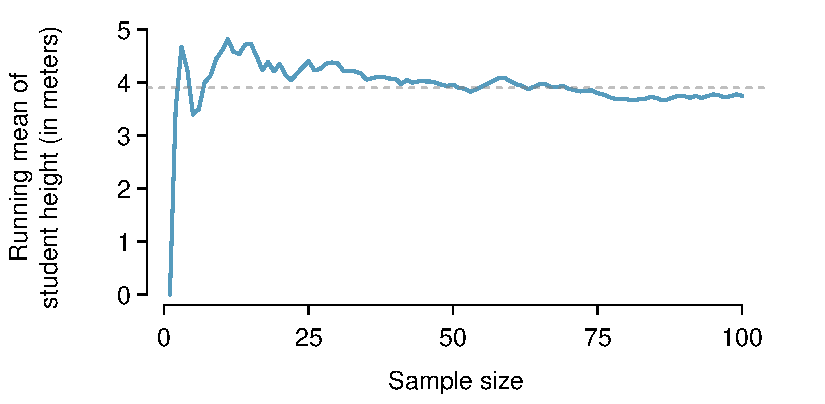
\includegraphics[width=0.72\textwidth]{ch_inference_foundations/figures/yrbssActiveRunningMean/yrbssActiveRunningMean}
   \caption{The mean computed after adding each individual to the sample. The mean tends to approach the true population average as more data become available.}
   \label{yrbssActiveRunningMean}
\end{figure}

Sample point estimates only approximate the population parameter, and they vary from one sample to another. If we took another simple random sample of the YRBSS students, we would find that the sample mean for the number of days active would be a little different. It will be useful to quantify how variable an estimate is from one sample to another. If this variability is small (i.e. the sample mean doesn't change much from one sample to another) then that estimate is probably very accurate. If it varies widely from one sample to another, then we should not expect our estimate to be very good.


\subsection{Standard error of the mean}
\label{seOfTheMean}

From the random sample represented in \data{yrbss\_samp}, we guessed the average number of days a YRBSS student is physically active is 3.75~days. Suppose we take another random sample of 100 individuals and take its mean: 3.22~days. Suppose we took another (3.67~days) and another (4.10~days), and so on. If we do this many many times -- which we can do only because we have all YRBSS students -- we can build up a \term{sampling distribution} for the sample mean when the sample size is 100, shown in Figure~\ref{yrbssActive1000SampDist}.

\begin{figure}[h]
   \centering
   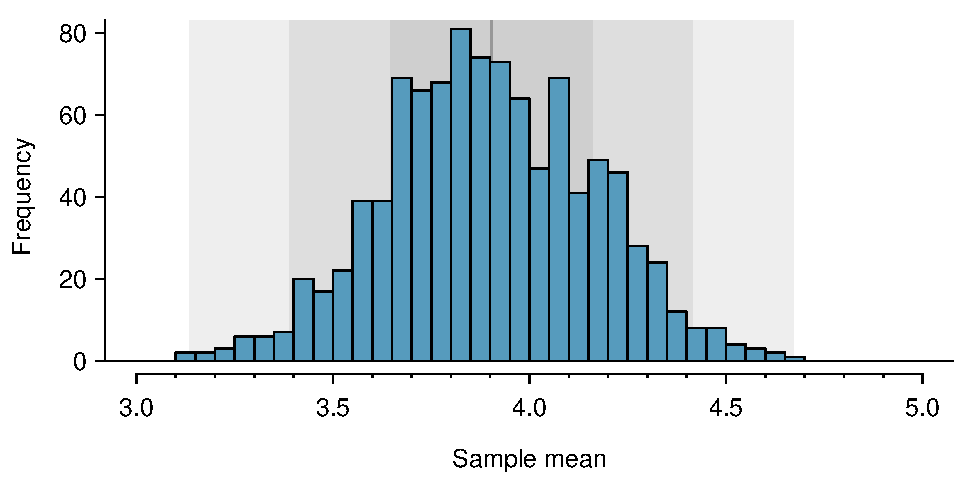
\includegraphics[width=0.9\textwidth]{ch_inference_foundations/figures/yrbssActive1000SampDist/yrbssActive1000SampDist}
   \caption{A histogram of 1000 sample means for number of days physically active per week, where the samples are of size $n=100$.}
   \label{yrbssActive1000SampDist}
\end{figure}

\begin{termBox}{\tBoxTitle{Sampling distribution}
The sampling distribution represents the distribution of the point estimates based on samples of a fixed size from a certain population. It is useful to think of a particular point estimate as being drawn from such a distribution. Understanding the concept of a sampling distribution is central to understanding statistical inference.}
\end{termBox}

The sampling distribution shown in Figure~\ref{yrbssActive1000SampDist} is unimodal and approximately symmetric. It is also centered exactly at the true population mean: $\mu=3.90$. Intuitively, this makes sense. The sample means should tend to ``fall around'' the population mean.

We can see that the sample mean has some variability around the population mean, which can be quantified using the standard deviation of this distribution of sample means: $\sigma_{\bar{x}} = 0.26$. The standard deviation of the sample mean tells us how far the typical estimate is away from the actual population mean, 3.90~days. It also describes the typical \term{error} of the point estimate, and for this reason we usually call this standard deviation the \term{standard error (SE)}\index{SE}\marginpar[\raggedright\vspace{-4mm}

$SE$\\\footnotesize standard\\error]{\raggedright\vspace{-4mm}

$SE$\\\footnotesize standard\\error} of the estimate.

\begin{termBox}{\tBoxTitle{Standard error of an estimate}
The standard deviation associated with an estimate is called the \emph{standard error}. It describes the typical error or uncertainty associated with the estimate.}
\end{termBox}

When considering the case of the point estimate $\bar{x}$, there is one problem: there is no obvious way to estimate its standard error from a single sample. However, statistical theory provides a helpful tool to address this issue. 

\textC{\newpage}

\begin{exercise}
(a) Would you rather use a small sample or a large sample when estimating a parameter? Why? (b) Using your reasoning from (a), would you expect a point estimate based on a small sample to have smaller or larger standard error than a point estimate based on a larger sample?\footnote{(a) Consider two random samples: one of size 10 and one of size 1000. Individual observations in the small sample are highly influential on the estimate while in larger samples these individual observations would more often average each other out. The larger sample would tend to provide a more accurate estimate. (b) If we think an estimate is better, we probably mean it typically has less error. Based on (a), our intuition suggests that a larger sample size corresponds to a smaller standard error.}
\end{exercise}

In the sample of 100 students, the standard error of the sample mean is equal to the population standard deviation divided by the square root of the sample size:
\begin{eqnarray*}
SE_{\bar{x}} = \sigma_{\bar{x}} = \frac{\sigma_{x}}{\sqrt{n}} = \frac{2.6}{\sqrt{100}} = 0.26
\end{eqnarray*}
where $\sigma_{x}$ is the standard deviation of the individual observations. This is no coincidence. We can show mathematically that this equation is correct when the observations are independent using the probability tools of Section~\ref{randomVariablesSection}.

\begin{termBox}{\tBoxTitle{Computing SE for the sample mean}
Given $n$ independent observations from a population with standard deviation $\sigma$, the standard error of the sample mean is equal to \vspace{-1mm}
\begin{eqnarray}
SE = \frac{\sigma}{\sqrt{n}}
\label{seOfXBar}
\end{eqnarray}\vspace{-3mm}%

A reliable method to ensure sample observations are independent is to conduct a simple random sample consisting of less than 10\% of the population.\index{standard error (SE)!single mean}
}
\end{termBox}

There is one subtle issue in Equation~(\ref{seOfXBar}): the population standard deviation is typically unknown. You might have already guessed how to resolve this problem: we can use the point estimate of the standard deviation from the sample. This estimate tends to be sufficiently good when the sample size is at least 30 and the population distribution is not strongly skewed%\footnote{Some books suggest 30 is sufficient; we take a slightly more conservative approach.}
% x <- c(); for(i in 1:10000){ x[i] <- mean(exp(rnorm(30, sd=0.5))) }; hist(x); (quantile(x, c(0.025, 0.975)) - mean(x)) / sd(x)
% M <- mean(x); x <- rep(NA, 1000); for(i in 1:1000){ temp <- exp(rnorm(30, sd=0.5)); x[i] <- (max(temp) - M) / sd(temp) }; hist(x); quantile(x, 0.95)
% for(i in 1:1000){ temp <- exp(rnorm(30, sd=0.5)); hist(temp, breaks=seq(0, 12, 0.5), main=round((max(temp) - mean(temp))/sd(temp), 1)); Sys.sleep(0.5) }
. Thus, we often just use the sample standard deviation $s$ instead of~$\sigma$. When the sample size is smaller than 30, we will need to use a method to account for extra uncertainty in the standard error. If the skew condition is not met, a larger sample is needed to compensate for the extra skew. These topics are further discussed in Section~\ref{cltSection}.

\begin{exercise}
In the sample of 100 students, the standard deviation of student heights is $s_{height} = 0.088$ meters. In this case, we can confirm that the observations are independent by checking that the data come from a simple random sample consisting of less than 10\% of the population. (a)~What is the standard error of the sample mean, $\bar{x}_{height} = 1.70$ meters? (b)~Would you be surprised if someone told you the average height of all YRBSS respondents was actually 1.69~meters?\footnote{(a) Use Equation~(\ref{seOfXBar}) with the sample standard deviation to compute the standard error: $SE_{\bar{y}} = 0.088 / \sqrt{100} = 0.0088$ meters. (b) It would not be surprising. Our sample is about 1 standard error from 1.69m. In other words, 1.69m does not seem to be implausible given that our sample was relatively close to it. (We use the standard error to identify what is close.)}
\end{exercise}
%library(openintro); library(xtable); data(yrbss); data(yrbss.samp); d <- yrbss.samp$height; mean(d); sd(d); mean(yrbss$height, na.rm=TRUE); sd(yrbss$height, na.rm=TRUE)

\textC{\pagebreak}

\begin{exercise}
(a) Would you be more trusting of a sample that has 100 observations or 400 observations? (b) We want to show mathematically that our estimate tends to be better when the sample size is larger. If the standard deviation of the individual observations is 10, what is our estimate of the standard error when the sample size is 100? What about when it is 400? (c) Explain how your answer to part~(b) mathematically justifies your intuition in part~(a).\footnote{(a) Extra observations are usually helpful in understanding the population, so a point estimate with 400 observations seems more trustworthy. (b) The standard error when the sample size is 100 is given by $SE_{100} = 10/\sqrt{100} = 1$. For 400: $SE_{400} = 10/\sqrt{400} = 0.5$. The larger sample has a smaller standard error. (c) The standard error of the sample with 400 observations is lower than that of the sample with 100 observations. The standard error describes the typical error, and since it is lower for the larger sample, this mathematically shows the estimate from the larger sample tends to be better -- though it does not guarantee that every large sample will provide a better estimate than a particular small sample.}
\end{exercise}

\subsection{Basic properties of point estimates}

We achieved three goals in this section. First, we determined that point estimates from a sample may be used to estimate population parameters. We also determined that these point estimates are not exact: they vary from one sample to another. Lastly, we quantified the uncertainty of the sample mean using what we call the standard error, mathematically represented in Equation~\eqref{seOfXBar}. While we could also quantify the standard error for other estimates -- such as the median, standard deviation, or any other number of statistics -- we will postpone these extensions until later chapters or courses.

\index{point estimate|)}


%__________________
\section[Confidence intervals]{Confidence intervals \sectionvideohref{youtube-FUaXoKdCre4&list=PLkIselvEzpM7Pjo94m1e7J5jkIZkbQAl4}}
\label{confidenceIntervals}

\index{confidence interval|(}

A point estimate provides a single plausible value for a parameter. However, a point estimate is rarely perfect; usually there is some error in the estimate. Instead of supplying just a point estimate of a parameter, a next logical step would be to provide a plausible \emph{range of values} for the parameter.

% In this section and in Section~\ref{hypothesisTesting}, we will emphasize the special case where the point estimate is a sample mean and the parameter is the population mean. In Section~\ref{aFrameworkForInference}, we generalize these methods for a variety of point estimates and population parameters that we will encounter in Chapter~\ref{inferenceForNumericalData} and beyond.

\subsection{Capturing the population parameter}

A plausible range of values for the population parameter is called a \term{confidence interval}.

Using only a point estimate is like fishing in a murky lake with a spear, and using a confidence interval is like fishing with a net. We can throw a spear where we saw a fish, but we will probably miss. On the other hand, if we toss a net in that area, we have a good chance of catching the fish.

If we report a point estimate, we probably will not hit the exact population parameter. On the other hand, if we report a range of plausible values -- a confidence interval -- we have a good shot at capturing the parameter. 

\begin{exercise}
If we want to be very certain we capture the population parameter, should we use a wider interval or a smaller interval?\footnote{If we want to be more certain we will capture the fish, we might use a wider net. Likewise, we use a wider confidence interval if we want to be more certain that we capture the parameter.}
\end{exercise}


\textC{\pagebreak}


\subsection{An approximate 95\% confidence interval}

Our point estimate is the most plausible value of the parameter, so it makes sense to build the confidence interval around the point estimate. The standard error, which is a measure of the uncertainty associated with the point estimate, provides a guide for how large we should make the confidence interval.

The standard error represents the standard deviation associated with the estimate, and roughly 95\% of the time the estimate will be within 2 standard errors of the parameter. If~the interval spreads out 2 standard errors from the point estimate, we can be roughly 95\% \term{confident} that we have captured the true parameter:
\begin{eqnarray}
\text{point estimate}\ \pm\ 2\times SE
\label{95PercentConfidenceIntervalFormula}
\end{eqnarray}
But what does ``95\% confident'' mean? Suppose we took many samples and built a confidence interval from each sample using Equation~(\ref{95PercentConfidenceIntervalFormula}). Then about 95\% of those intervals would contain the actual mean, $\mu$. Figure~\ref{95PercentConfidenceInterval} shows this process with 25 samples, where 24 of the resulting confidence intervals contain the average number of days per week that YRBSS students are physically active, $\mu=3.90$~days, and one interval does not.

\begin{figure}[hht]
   \centering
   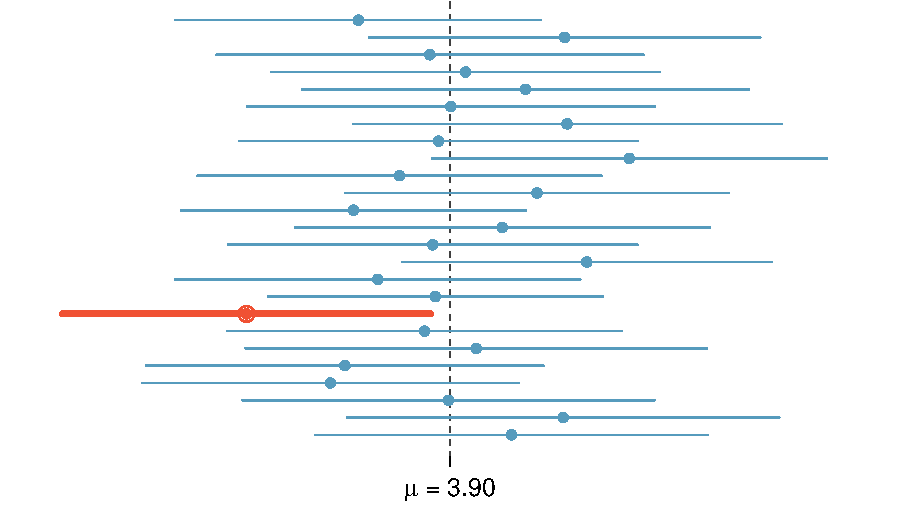
\includegraphics[width=0.78\textwidth]{ch_inference_foundations/figures/95PercentConfidenceInterval/95PercentConfidenceInterval}
   \caption{Twenty-five samples of size $n=100$ were taken from \data{yrbss}. For~each sample, a confidence interval was created to try to capture the average number of days per week that students are physically active. Only~1 of these~25 intervals did not capture the true mean, $\mu = 3.90$~days.}
   \label{95PercentConfidenceInterval}
\end{figure}

\begin{exercise}
In Figure~\ref{95PercentConfidenceInterval}, one interval does not contain 3.90 minutes. Does this imply that the mean cannot be 3.90?\footnote{Just as some observations occur more than 2 standard deviations from the mean, some point estimates will be more than 2 standard errors from the parameter. A confidence interval only provides a plausible range of values for a parameter. While we might say other values are implausible based on the data, this does not mean they are impossible.}
\end{exercise}

The rule where about 95\% of observations are within 2 standard deviations of the mean is only approximately true. However, it holds very well for the normal distribution. As we will soon see, the mean tends to be normally distributed when the sample size is sufficiently large. 

\begin{example}{The sample mean of days active per week from \data{yrbss\_samp} is 3.75~days. The standard error, as estimated using the sample standard deviation, is $SE=\frac{2.6}{\sqrt{100}} = 0.26$~days. (The population SD is unknown in most applications, so we use the sample SD here.) Calculate an approximate 95\% confidence interval for the average days active per week for all YRBSS students.}
We apply Equation~(\ref{95PercentConfidenceIntervalFormula}):
\begin{eqnarray*}
3.75\ \pm\ 2 \times  0.26 \quad \rightarrow \quad (3.23, 4.27)
\end{eqnarray*}
Based on these data, we are about 95\% confident that the average days active per week for all YRBSS students was larger than 3.23 but less than 4.27~days. Our~interval extends out 2 standard errors from the point estimate, $\bar{x}_{active}$.
\end{example}
% library(openintro); library(xtable); d <- yrbss.samp; mean(d$physically_active_7d); sd(d$physically_active_7d); sd(yrbss$physically_active_7d, na.rm=TRUE)

\begin{exercise} \label{95CIExerciseForAgeOfYrbssSamp1}
The sample data suggest the average YRBSS student height is $\bar{x}_{height} = 1.697$ meters with a standard error of 0.0088 meters (estimated using the sample standard deviation, 0.088 meters). What is an approximate 95\% confidence interval for the average height of all of the YRBSS students?\footnote{Apply Equation~(\ref{95PercentConfidenceIntervalFormula}): $1.697 \ \pm \ 2\times 0.0088 \rightarrow (1.6794, 1.7146)$. We interpret this interval as follows: We are about 95\% confident the average height of all YRBSS students was between 1.6794 and 1.7146 meters (5.51~to 5.62~feet).}
\end{exercise}
% library(openintro); d <- yrbss.samp; mean(d$height); sd(d$height)

\subsection{The sampling distribution for the mean}

In Section~\ref{seOfTheMean}, we introduced a sampling distribution for $\bar{x}$, the average days physically active per week for samples of size 100. We examined this distribution earlier in Figure~\ref{yrbssActive1000SampDist}. Now we'll take 100,000 samples, calculate the mean of each, and plot them in a histogram to get an especially accurate depiction of the sampling distribution. This histogram is shown in the left panel of Figure~\ref{yrbssActiveBigSampDist}.

\begin{figure}[hht]
   \centering
   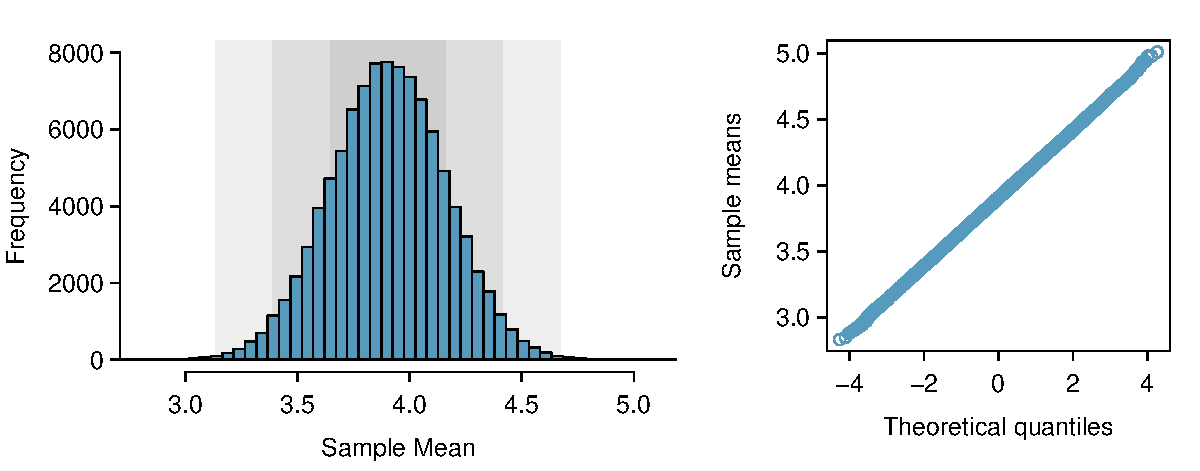
\includegraphics[width=\textwidth]{ch_inference_foundations/figures/yrbssActiveBigSampDist/yrbssActiveBigSampDist}
   \caption{The left panel shows a histogram of the sample means for 100,000 different random samples. The right panel shows a normal probability plot of those sample means.}
   \label{yrbssActiveBigSampDist}
\end{figure}

Does this distribution look familiar? Hopefully so! The distribution of sample means closely resembles the normal distribution (see Section~\ref{normalDist}). A normal probability plot of these sample means is shown in the right panel of Figure~\ref{yrbssActiveBigSampDist}. Because all of the points closely fall around a straight line, we can conclude the distribution of sample means is nearly normal. This result can be explained by the Central Limit Theorem.

\begin{termBox}{\tBoxTitle{Central Limit Theorem, informal description}
If a sample consists of at least 30 independent observations and the data are not strongly skewed, then the distribution of the sample mean is well approximated by a~normal model.\index{Central Limit Theorem}}
\end{termBox}

We will apply this informal version of the Central Limit Theorem for now, and discuss its details further in Section~\ref{cltSection}.

The choice of using 2 standard errors in Equation~(\ref{95PercentConfidenceIntervalFormula}) was based on our general guideline that roughly 95\% of the time, observations are within two standard deviations of the mean. Under the normal model, we can make this more accurate by using 1.96 in place~of~2.
\begin{eqnarray}
\text{point estimate}\ \pm\ 1.96\times SE
\label{95PercentCIWhenUsingNormalModel}
\end{eqnarray}
If a point estimate, such as $\bar{x}$, is associated with a normal model and standard error $SE$, then we use this more precise 95\% confidence interval.


\subsection{Changing the confidence level}
\label{changingTheConfidenceLevelSection}

\index{confidence interval!confidence level|(}

Suppose we want to consider confidence intervals where the confidence level is somewhat higher than 95\%; perhaps we would like a confidence level of 99\%. Think back to the analogy about trying to catch a fish: if we want to be more sure that we will catch the fish, we should use a wider net. To create a 99\% confidence level, we must also widen our 95\% interval. On the other hand, if we want an interval with lower confidence, such as 90\%, we could make our original 95\% interval slightly slimmer.

The 95\% confidence interval structure provides guidance in how to make intervals with new confidence levels. Below is a general 95\% confidence interval for a point estimate that comes from a nearly normal distribution:
\begin{eqnarray}
\text{point estimate}\ \pm\ 1.96\times SE
\end{eqnarray}
There are three components to this interval: the point estimate, ``1.96'', and the standard error. The choice of $1.96\times SE$ was based on capturing 95\% of the data since the estimate is within 1.96 standard deviations of the parameter about 95\% of the time. The choice of 1.96 corresponds to a 95\% confidence level. 

\begin{exercise} \label{leadInForMakingA99PercentCIExercise}
If $X$ is a normally distributed random variable, how often will $X$ be within 2.58 standard deviations of the mean?\footnote{This is equivalent to asking how often the Z-score will be larger than -2.58 but less than 2.58. (For a picture, see Figure~\ref{choosingZForCI}.) To determine this probability, look up -2.58 and 2.58 in the normal probability table (0.0049 and 0.9951). Thus, there is a $0.9951-0.0049 \approx 0.99$ probability that the unobserved random variable $X$ will be within 2.58 standard deviations of $\mu$.}
\end{exercise}

To create a 99\% confidence interval, change 1.96 in the 95\% confidence interval formula to be $2.58$. Guided Practice~\ref{leadInForMakingA99PercentCIExercise} highlights that 99\% of the time a normal random variable will be within 2.58 standard deviations of the mean. This approach -- using the Z-scores in the normal model to compute confidence levels -- is appropriate when $\bar{x}$ is associated with a normal distribution with mean $\mu$ and standard deviation $SE_{\bar{x}}$. Thus, the formula for a 99\% confidence interval is
\begin{eqnarray}
\bar{x}\ \pm\ 2.58\times SE_{\bar{x}}
\label{99PercCIForMean}
\end{eqnarray}

\begin{figure}[h]
\centering
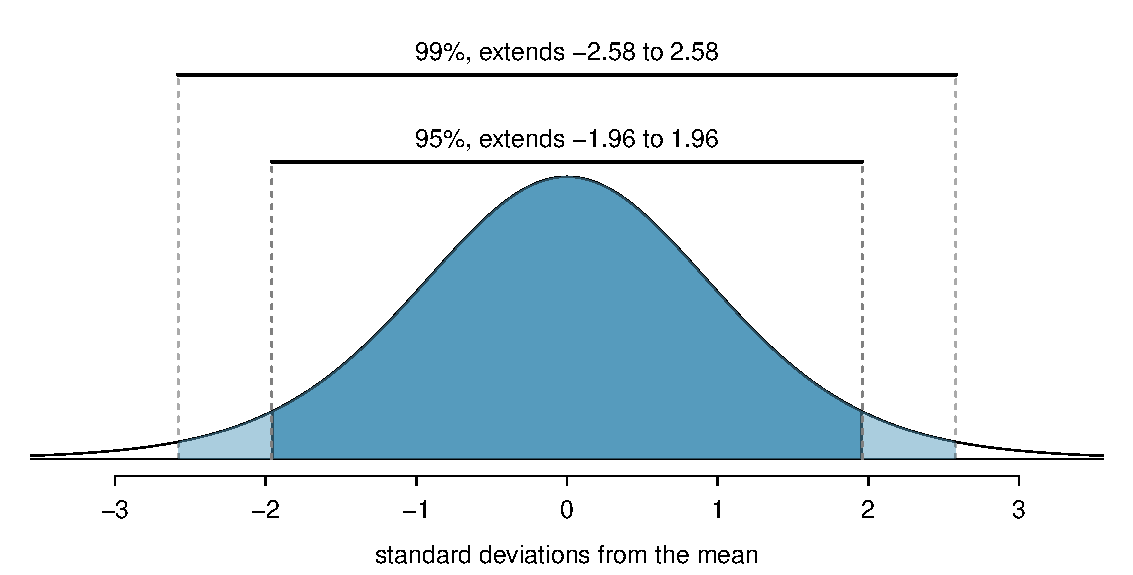
\includegraphics[width=\textwidth]{ch_inference_foundations/figures/choosingZForCI/choosingZForCI}
\caption{The area between -$z^{\star}$ and $z^{\star}$ increases as $|z^{\star}|$ becomes larger. If the confidence level is 99\%, we choose $z^{\star}$ such that 99\% of the normal curve is between -$z^{\star}$ and $z^{\star}$, which corresponds to 0.5\% in the lower tail and 0.5\% in the upper tail: $z^{\star}=2.58$.}
\label{choosingZForCI}
\index{confidence interval!confidence level|)}
\end{figure}

The normal approximation is crucial to the precision of these confidence intervals. Section~\ref{cltSection} provides a more detailed discussion about when the normal model can safely be applied. When the normal model is not a good fit, we will use alternative distributions that better characterize the sampling distribution.

\begin{termBox}{\tBoxTitle{Conditions for $\bar{x}$ being nearly normal and $SE$ being accurate\label{terBoxOfCondForXBarBeingNearlyNormalAndSEBeingAccurate}}
Important conditions to help ensure the sampling distribution of $\bar{x}$ is nearly normal and the estimate of SE sufficiently accurate:
\begin{itemize}
\setlength{\itemsep}{0mm}
\item The sample observations are independent.
\item The sample size is large: $n\geq30$ is a good rule of thumb.
\item The population distribution is not strongly skewed. This condition can be difficult to evaluate, so just use your best judgement.
\end{itemize}
Additionally, the larger the sample size, the more lenient we can be with the sample's skew.}
\end{termBox}

\begin{tipBox}{\tipBoxTitle[]{How to verify sample observations are independent}
If the observations are from a simple random sample and consist of fewer than 10\% of the population, then they are independent.\\[2mm]
Subjects in an experiment are considered independent if they undergo random assignment to the treatment groups. \\[2mm]
If a sample is from a seemingly random process, e.g. the lifetimes of wrenches used in a particular manufacturing process, checking independence is more difficult. In~this case, use your best judgement.}
\end{tipBox}

\begin{tipBox}{\tipBoxTitle[]{Checking for strong skew usually means checking for obvious outliers}
When there are prominent outliers present, the sample should contain at least 100 observations, and in some cases, much more. \\[2mm]
This is a first course in statistics, so you won't have perfect judgement on assessing skew. That's okay. If you're in a bind, either consult a statistician or learn about the studentized bootstrap (bootstrap-t) method.}
\end{tipBox}

% WARNING !!!!
% EOCE 4.9 (as of 2nd Edition) references the results of this exercise
\begin{exercise} \label{find99CIForYrbssAgeExercise}
Create a 99\% confidence interval for the average days active per week of all YRBSS students using \data{yrbss\_samp}. The point estimate is $\bar{x}_{active} = 3.75$ and the standard error is $SE_{\bar{x}} = 0.26$.\footnote{The observations are independent (simple random sample, $<10\%$ of the population), the sample size is at least 30 ($n = 100$), and the distribution doesn't have a clear skew (Figure~\ref{yrbssSampHistograms} on page~\pageref{yrbssSampHistograms}); the normal approximation and estimate of SE should be reasonable. Apply the 99\% confidence interval formula: $\bar{x}_{active}\ \pm\ 2.58 \times  SE_{\bar{x}} \rightarrow (3.08, 4.42)$. We are 99\% confident that the average days active per week of all YRBSS students is between 3.08 and 4.42~days.}
\end{exercise}
%library(openintro); data(yrbss.samp); d <- yrbss.samp; mean(d$age); sd(d$age)/sqrt(100)

\begin{termBox}{\tBoxTitle{Confidence interval for any confidence level}
If the point estimate follows the normal model with standard error $SE$, then a confidence interval for the population parameter is
\begin{eqnarray*}
\text{point estimate}\ \pm\ z^{\star} SE
\end{eqnarray*}
where $z^{\star}$ corresponds to the confidence level selected.}
\end{termBox}

Figure~\ref{choosingZForCI} provides a picture of how to identify $z^{\star}$ based on a confidence level. We~select $z^{\star}$ so that the area between -$z^{\star}$ and $z^{\star}$ in the normal model corresponds to the confidence level. 

\begin{termBox}{\tBoxTitle{Margin of error}
\label{marginOfErrorTermBox}In a confidence interval, $z^{\star}\times SE$ is called the \term{margin of error}.}
\end{termBox}

\textC{\newpage}

\begin{exercise} \label{find90CIForYrbssAgeExercise}
Use the data in Guided Practice~\ref{find99CIForYrbssAgeExercise} to create a 90\% confidence interval for the average days active per week of all YRBSS students.\footnote{We first find $z^{\star}$ such that 90\% of the distribution falls between -$z^{\star}$ and $z^{\star}$ in the standard normal model, $N(\mu=0, \sigma=1)$. We can look up -$z^{\star}$ in the normal probability table by looking for a lower tail of 5\% (the other 5\% is in the upper tail): $z^{\star}=1.65$. The 90\% confidence interval can then be computed as $\bar{x}_{active}\ \pm\ 1.65\times SE_{\bar{x}} \to (3.32, 4.18)$. (We had already verified conditions for normality and the standard error.) That is, we are 90\% confident the average days active per week is between 3.32 and 4.18~days.}
\end{exercise}

\subsection{Interpreting confidence intervals}
\label{interpretingCIs}

\index{confidence interval!interpretation|(}

A careful eye might have observed the somewhat awkward language used to describe confidence intervals. Correct interpretation:
\begin{quote}
We are XX\% confident that the population parameter is between...
\end{quote}
\emph{Incorrect} language might try to describe the confidence interval as capturing the population parameter with a certain probability. This is a common error: while it might be useful to think of it as a probability, the confidence level only quantifies how plausible it is that the parameter is in the interval.

Another important consideration of confidence intervals is that they \emph{only try to capture the population parameter}. A confidence interval says nothing about the confidence of capturing individual observations, a proportion of the observations, or about capturing point estimates. Confidence intervals only attempt to capture population parameters.

\index{confidence interval!interpretation|)}
\index{confidence interval|)}



%__________________
\section[Hypothesis testing]{Hypothesis testing \sectionvideohref{youtube-NVbPE1_Cbx8&list=PLkIselvEzpM7Pjo94m1e7J5jkIZkbQAl4}}
\label{hypothesisTesting}

\index{hypothesis testing|(}

Are students lifting weights or performing other strength training exercises more or less often than they have in the past? We'll compare data from students from the 2011 YRBSS survey to our sample of 100 students from the 2013 YRBSS survey.

We'll also consider sleep behavior. A recent study found that college students average about 7~hours of sleep per night.\footnote{\oiRedirect{textbook-theloquitur_1161}{\emph{Poll shows college students get least amount of sleep}. theloquitur.com/?p=1161}} However, researchers at a rural college are interested in showing that their students sleep longer than seven hours on average. We investigate this topic in Section~\ref{pValue}.

\subsection{Hypothesis testing framework}

Students from the 2011 YRBSS lifted weights (or performed other strength training exercises) 3.09~days per week on average. We want to determine if the \data{yrbss\_samp} data set provides strong evidence that YRBSS students selected in 2013 are lifting more or less than the 2011 YRBSS students, versus the other possibility that there has been no change.\footnote{While we could answer this question by examining the entire YRBSS data set from 2013 (\data{yrbss}), we only consider the sample data (\data{yrbss\_samp}), which is more realistic since we rarely have access to population data.} We simplify these three options into two competing \termsub{hypotheses}{hypothesis}:
\begin{itemize}
\setlength{\itemsep}{0mm}
\item[$H_0$:] The average days per week that YRBSS students lifted weights was the same for 2011 and~2013.
\item[$H_A$:] The average days per week that YRBSS students lifted weights was \emph{different} for 2013 than~in~2011.
\end{itemize}
We call $H_0$\marginpar[\raggedright\vspace{6mm}

$H_0$\\\footnotesize null hypothesis\vspace{3mm}\\\normalsize $H_A$\\\footnotesize alternative\\ hypothesis]{\raggedright\vspace{6mm}

$H_0$\\\footnotesize null hypothesis\vspace{3mm}\\\normalsize $H_A$\\\footnotesize alternative\\ hypothesis} the null hypothesis and $H_A$ the alternative hypothesis.

\begin{termBox}{\tBoxTitle{Null and alternative hypotheses}
{\small The \term{null hypothesis ($H_0$)} often represents either a skeptical perspective or a claim to be tested. The \term{alternative hypothesis ($H_A$)} represents an alternative claim under consideration and is often represented by a range of possible parameter values.}}
\end{termBox}

The null hypothesis often represents a skeptical position or a perspective of no difference. The alternative hypothesis often represents a new perspective, such as the possibility that there has been a change. 

\begin{tipBox}{\tipBoxTitle{Hypothesis testing framework}
The skeptic will not reject the null hypothesis ($H_0$), unless the evidence in favor of the alternative hypothesis ($H_A$) is so strong that she rejects $H_0$ in favor of $H_A$.}
\end{tipBox}

The hypothesis testing framework is a very general tool, and we often use it without a second thought. If a person makes a somewhat unbelievable claim, we are initially skeptical. However, if there is sufficient evidence that supports the claim, we set aside our skepticism and reject the null hypothesis in favor of the alternative. The hallmarks of hypothesis testing are also found in the US court system. 

\begin{exercise} \label{hypTestCourtExample}
A US court considers two possible claims about a defendant: she is either innocent or guilty. If we set these claims up in a hypothesis framework, which would be the null hypothesis and which the alternative?\footnote{The jury considers whether the evidence is so convincing (strong) that there is no reasonable doubt regarding the person's guilt; in such a case, the jury rejects innocence (the null hypothesis) and concludes the defendant is guilty (alternative hypothesis).}
\end{exercise}

Jurors examine the evidence to see whether it convincingly shows a defendant is guilty. Even if the jurors leave unconvinced of guilt beyond a reasonable doubt, this does not mean they believe the defendant is innocent. This is also the case with hypothesis testing: \emph{even if we fail to reject the null hypothesis, we typically do not accept the null hypothesis as true}. Failing to find strong evidence for the alternative hypothesis is not equivalent to accepting the null hypothesis.

In the example with the YRSS, the null hypothesis represents no difference in the average days per week of weight lifting in 2011 and 2013. The alternative hypothesis represents something new or more interesting: there was a difference, either an increase or a decrease. These hypotheses can be described in mathematical notation using $\mu_{13}$ as the average days of weight lifting for 2013:
\begin{itemize}
\setlength{\itemsep}{0mm}
\item[$H_0$:] $\mu_{13} = 3.09$
\item[$H_A$:] $\mu_{13} \neq 3.09$
\end{itemize}
where 3.09 is the average number of days per week that students from the 2011 YRBSS lifted weights. Using the mathematical notation, the hypotheses can more easily be evaluated using statistical tools. We call 3.09 the \term{null value} since it represents the value of the parameter if the null hypothesis is true.


\subsection{Testing hypotheses using confidence intervals}
\label{utilizingOurCI}

We will use the \data{yrbss\_samp} data set to evaluate the hypothesis test, and we start by comparing the 2013 point estimate of the number of days per week that students lifted weights: $\bar{x}_{13} = 2.78$~days. This estimate suggests that students from the 2013 YRBSS were lifting weights less than students in the 2011 YRBSS. However, to evaluate whether this provides strong evidence that there has been a change, we must consider the uncertainty associated with $\bar{x}_{13}$.

We learned in Section~\ref{variabilityInEstimates} that there is fluctuation from one sample to another, and it is unlikely that the sample mean will be exactly equal to the parameter; we should not expect $\bar{x}_{13}$ to exactly equal $\mu_{13}$. Given that $\bar{x}_{13} = 2.78$, it might still be possible that the average of all students from the 2013 YRBSS survey is the same as the average from the 2011 YRBSS survey. The difference between $\bar{x}_{13}$ and 3.09 could be due to \emph{sampling variation}, i.e. the variability associated with the point estimate when we take a random sample.

In Section~\ref{confidenceIntervals}, confidence intervals were introduced as a way to find a range of plausible values for the population mean.

\begin{example}{In the sample of 100 students from the 2013 YRBSS survey, the average number of days per week that students lifted weights was 2.78~days with a standard deviation of 2.56 days (coincidentally the same as days active). Compute a 95\% confidence interval for the average for all students from the 2013 YRBSS survey. You can assume the conditions for the normal model are met.}
The general formula for the confidence interval based on the normal distribution is
\begin{align*}
\bar{x} \pm z^{\star} SE_{\bar{x}}
\end{align*}
We are given $\bar{x}_{13} = 2.78$, we use $z^{\star} = 1.96$ for a 95\% confidence level, and we can compute the standard error using the standard deviation divided by the square root of the sample size:
\begin{align*}
SE_{\bar{x}} = \frac{s_{13}}{\sqrt{n}} = \frac{2.56}{\sqrt{100}} = 0.256
\end{align*}
Entering the sample mean, $z^{\star}$, and the standard error into the confidence interval formula results in (2.27, 3.29). We are 95\% confident that the average number of days per week that all students from the 2013 YRBSS lifted weights was between 2.27~and 3.29~days.
\end{example}

Because the average of all students from the 2013 YRBSS survey is 3.09, which falls within the range of plausible values from the confidence interval, we cannot say the null hypothesis is implausible. That is, we fail to reject the null hypothesis, $H_0$.

\begin{tipBox}{\tipBoxTitle{Double negatives can sometimes be used in statistics}
In many statistical explanations, we use double negatives. For instance, we might say that the null hypothesis is \emph{not implausible} or we \emph{failed to reject} the null hypothesis. Double negatives are used to communicate that while we are not rejecting a position, we are also not saying it is correct.}
\end{tipBox}

\begin{exercise} \label{htForHousingExpenseForCommunityCollege650}
Colleges frequently provide estimates of student expenses such as housing. A consultant hired by a community college claimed that the average student housing expense was \$650 per month. What are the null and alternative hypotheses to test whether this claim is accurate?\footnote{$H_0$: The average cost is \$650 per month, $\mu = \$650$.

\hspace{3.4mm}$H_A$: The average cost is different than \$650 per month, $\mu \neq \$650$.}
\end{exercise}

\begin{exercise} \label{normalDistCondForHousingExpenseForCommunityCollege650}
The community college decides to collect data to evaluate the \$650 per month claim. They take a random sample of 175 students at their school and obtain the data represented in Figure~\ref{communityCollegeClaimedHousingExpenseDistribution}. Can we apply the normal model to the sample mean?\footnote{Applying the normal model requires that certain conditions are met. Because the data are a simple random sample and the sample (presumably) represents no more than 10\% of all students at the college, the observations are independent. The sample size is also sufficiently large ($n = 175$) and the data exhibit strong skew. While the data are strongly skewed, the sample is sufficiently large that this is acceptable, and the normal model may be applied to the sample mean.}

\begin{figure}
\centering
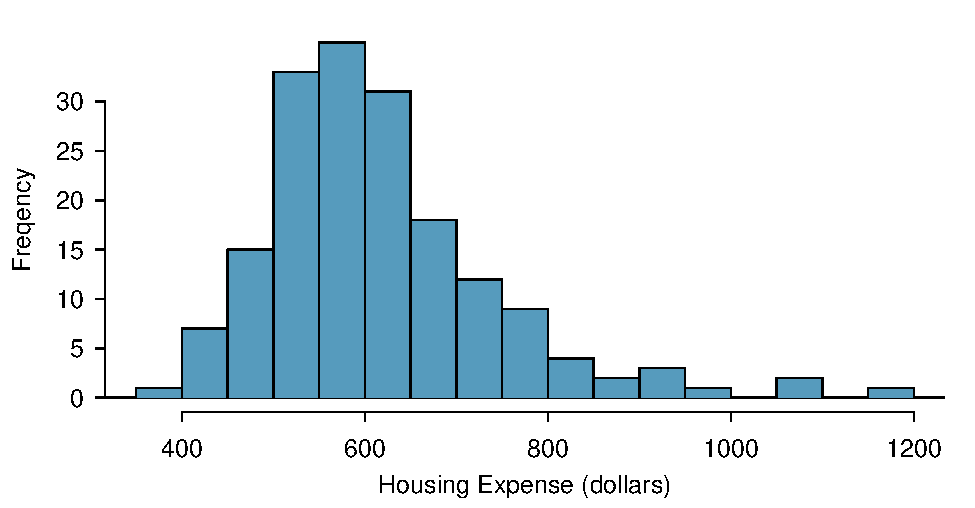
\includegraphics[width=0.9\textwidth]{ch_inference_foundations/figures/communityCollegeClaimedHousingExpenseDistribution/communityCollegeClaimedHousingExpenseDistribution}
\caption{Sample distribution of student housing expense. These data are strongly skewed\index{skew!example: strong}, which we can see by the long right tail with a few notable outliers.}
\label{communityCollegeClaimedHousingExpenseDistribution}
\end{figure}
\end{exercise}

\begin{tipBox}{\tipBoxTitle[]{Evaluating the skew condition is challenging}
Don't despair if checking the skew condition is difficult or confusing. You aren't alone -- nearly all students get frustrated when checking skew. Properly assessing skew takes practice, and you won't be a pro, even at the end of this book. \\[2mm]
But this doesn't mean you should give up. Checking skew and the other conditions is extremely important for a responsible data analysis. However, rest assured that evaluating skew isn't something you need to be a master of by the end of the book, though by that time you should be able to properly assess clear cut cases.}
\end{tipBox}

\textC{\newpage}

\begin{example}{The sample mean for student housing is \$616.91 and the sample standard deviation is \$128.65. Construct a 95\% confidence interval for the population mean and evaluate the hypotheses of Guided Practice~\ref{htForHousingExpenseForCommunityCollege650}.}
The standard error associated with the mean may be estimated using the sample standard deviation divided by the square root of the sample size. Recall that $n = 175$ students were sampled.
\begin{align*}
SE = \frac{s}{\sqrt{n}} = \frac{128.65}{\sqrt{175}} = 9.73
\end{align*}
You showed in Guided Practice~\ref{normalDistCondForHousingExpenseForCommunityCollege650} that the normal model may be applied to the sample mean. This ensures a 95\% confidence interval may be accurately constructed:
$$\bar{x}\ \pm\ z^{\star} SE \quad\to\quad 616.91\ \pm\ 1.96 \times 9.73 \quad \to \quad (597.84, 635.98) $$
Because the null value \$650 is not in the confidence interval, a true mean of \$650 is implausible and we reject the null hypothesis. The data provide statistically significant evidence that the actual average housing expense is less than \$650 per month.
\end{example}


\subsection{Decision errors}

\index{hypothesis testing!decision errors|(}

Hypothesis tests are not flawless, since we can make a wrong decision in statistical hypothesis tests based on the data. For example, in the court system innocent people are sometimes wrongly convicted and the guilty sometimes walk free. However, the difference is that in statistical hypothesis tests, we have the tools necessary to quantify how often we make such errors.

% Hypothesis tests are not flawless. Just think of the court system: innocent people are sometimes wrongly convicted and the guilty sometimes walk free. Similarly, we can make a wrong decision in statistical hypothesis tests. However, the difference is that we have the tools necessary to quantify how often we make such errors.

There are two competing hypotheses: the null and the alternative. In a hypothesis test, we make a statement about which one might be true, but we might choose incorrectly. There are four possible scenarios, which are summarized in Table~\ref{fourHTScenarios}.

\begin{table}[ht]
\centering
\begin{tabular}{l l c c}
& & \multicolumn{2}{c}{\textbf{Test conclusion}} \\
  \cline{3-4}
\vspace{-3.7mm} \\
& & do not reject $H_0$ &  reject $H_0$ in favor of $H_A$ \\
  \cline{2-4}
\vspace{-3.7mm} \\
& $H_0$ true & okay &  Type~1 Error \\
\raisebox{1.5ex}{\textbf{Truth}} & $H_A$ true & Type~2 Error & okay \\
  \cline{2-4}
\end{tabular}
\caption{Four different scenarios for hypothesis tests.}
\label{fourHTScenarios}
\end{table}

A \term{Type~1 Error} is rejecting the null hypothesis when $H_0$ is actually true. A \term{Type~2 Error} is failing to reject the null hypothesis when the alternative is actually true.

\begin{exercise} \label{whatAreTheErrorTypesInUSCourts}
In a US court, the defendant is either innocent ($H_0$) or  guilty ($H_A$). What does a Type~1 Error represent in this context? What does a Type~2 Error represent? Table~\ref{fourHTScenarios} may be useful.\footnote{If the court makes a Type~1 Error, this means the defendant is innocent ($H_0$ true) but wrongly convicted. A Type~2 Error means the court failed to reject $H_0$ (i.e. failed to convict the person) when she was in fact guilty ($H_A$ true).}
\end{exercise}

\begin{exercise} \label{howToReduceType1ErrorsInUSCourts}
How could we reduce the Type~1 Error rate in US courts? What influence would this have on the Type~2 Error rate?\footnote{To lower the Type~1 Error rate, we might raise our standard for conviction from ``beyond a reasonable doubt'' to ``beyond a conceivable doubt'' so fewer people would be wrongly convicted. However, this would also make it more difficult to convict the people who are actually guilty, so we would make more Type~2 Errors.}
\end{exercise}

\begin{exercise} \label{howToReduceType2ErrorsInUSCourts}
How could we reduce the Type~2 Error rate in US courts? What influence would this have on the Type~1 Error rate?\footnote{To lower the Type~2 Error rate, we want to convict more guilty people. We could lower the standards for conviction from ``beyond a reasonable doubt'' to ``beyond a little doubt''. Lowering the bar for guilt will also result in more wrongful convictions, raising the Type~1 Error rate.}
\end{exercise}

\index{hypothesis testing!decision errors|)}

Exercises~\ref{whatAreTheErrorTypesInUSCourts}-\ref{howToReduceType2ErrorsInUSCourts} provide an important lesson: if we reduce how often we make one type of error, we generally make more of the other type.

Hypothesis testing is built around rejecting or failing to reject the null hypothesis. That is, we do not reject $H_0$ unless we have strong evidence. But what precisely does \emph{strong evidence} mean? As a general rule of thumb, for those cases where the null hypothesis is actually true, we do not want to incorrectly reject $H_0$ more than 5\% of the time. This corresponds to a \term{significance level}\index{hypothesis testing!significance level} of 0.05. We often write the significance level using $\alpha$\marginpar[\raggedright\vspace{-4mm}

$\alpha$\\\footnotesize significance\\level of a\\hypothesis test]{\raggedright\vspace{-4mm}

$\alpha$\\\footnotesize significance\\level of a\\hypothesis test} (the Greek letter \emph{alpha}\index{Greek!alpha@alpha ($\alpha$)}): $\alpha = 0.05$. We discuss the appropriateness of different significance levels in Section~\ref{significanceLevel}.

If we use a 95\% confidence interval to evaluate a hypothesis test where the null hypothesis is true, we will make an error whenever the point estimate is at least 1.96 standard errors away from the population parameter. This happens about 5\% of the time (2.5\% in each tail). Similarly, using a 99\% confidence interval to evaluate a hypothesis is equivalent to a significance level of $\alpha = 0.01$.

A confidence interval is, in one sense, simplistic in the world of hypothesis tests. Consider the following two scenarios:
\begin{itemize}
\setlength{\itemsep}{0mm}
\item The null value (the parameter value under the null hypothesis) is in the 95\% confidence interval but just barely, so we would not reject $H_0$. However, we might like to somehow say, quantitatively, that it was a close decision.
\item The null value is very far outside of the interval, so we reject $H_0$. However, we want to communicate that, not only did we reject the null hypothesis, but it wasn't even close. Such a case is depicted in Figure~\ref{whyWeWantPValue}.
\end{itemize}
In Section~\ref{pValue}, we introduce a tool called the \emph{p-value} that will be helpful in these cases. The p-value method also extends to hypothesis tests where confidence intervals cannot be easily constructed or applied.

\begin{figure}[hht]
\centering
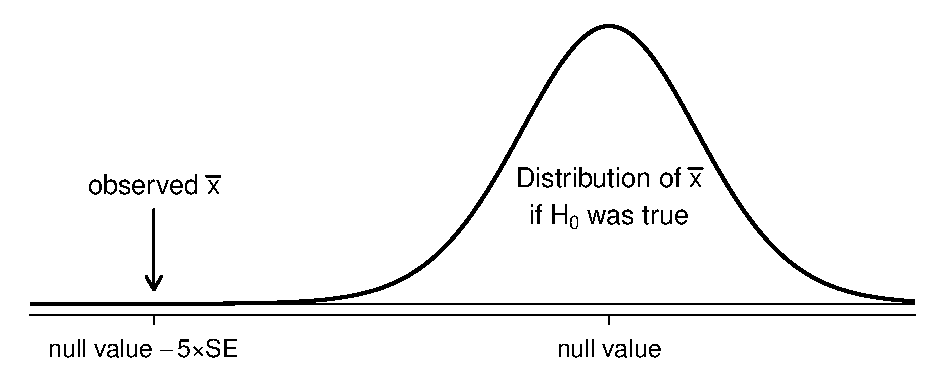
\includegraphics[width=0.75\textwidth]{ch_inference_foundations/figures/whyWeWantPValue/whyWeWantPValue}
\caption{It would be helpful to quantify the strength of the evidence against the null hypothesis. In this case, the evidence is extremely strong.}
\label{whyWeWantPValue}
\end{figure}


\subsection{Formal testing using p-values}
\label{pValue}

\index{hypothesis testing!p-value|(}

The p-value is a way of quantifying the strength of the evidence against the null hypothesis and in favor of the alternative. Formally the \emph{p-value} is a conditional probability.

\begin{termBox}{\tBoxTitle{p-value}
The \term{p-value}\index{hypothesis testing!p-value|textbf} is the probability of observing data at least as favorable to the alternative hypothesis as our current data set, if the null hypothesis is true. We typically use a summary statistic of the data, in this chapter the sample mean, to help compute the p-value and evaluate the hypotheses.}
\end{termBox}

\index{data!school sleep|(}


\begin{exercise} \label{skepticalPerspOfRuralSchoolSleepExercise}
A poll by the National Sleep Foundation found that college students average about 7 hours of sleep per night. Researchers at a rural school are interested in showing that students at their school sleep longer than seven hours on average, and they would like to demonstrate this using a sample of students. What would be an appropriate skeptical position for this research?\footnote{A skeptic would have no reason to believe that sleep patterns at this school are different than the sleep patterns at another school.}
\end{exercise}

We can set up the null hypothesis for this test as a skeptical perspective: the students at this school average 7 hours of sleep per night. The alternative hypothesis takes a new form reflecting the interests of the research: the students average more than 7 hours of sleep. We can write these hypotheses as
\begin{itemize}
\setlength{\itemsep}{0mm}
\item[$H_0$:] $\mu = 7$.
\item[$H_A$:] $\mu > 7$.
\end{itemize}
Using $\mu > 7$ as the alternative is an example of a \term{one-sided} hypothesis test. In this investigation, there is no apparent interest in learning whether the mean is less than 7~hours.\footnote{This is entirely based on the interests of the researchers. Had they been only interested in the opposite case -- showing that their students were actually averaging fewer than seven hours of sleep but not interested in showing more than 7 hours -- then our setup would have set the alternative as $\mu < 7$.} Earlier we encountered a \term{two-sided} hypothesis where we looked for any clear difference, greater than or less than the null value.

Always use a two-sided test unless it was made clear prior to data collection that the test should be one-sided. Switching a two-sided test to a one-sided test after observing the data is dangerous because it can inflate the Type~1 Error rate. 

\begin{tipBox}{\tipBoxTitle{One-sided and two-sided tests}
When you are interested in checking for an increase or a decrease, but not both, use a one-sided test. When you are interested in any difference from the null value~--~an increase or decrease~--~then the test should be two-sided.\vspace{0.5mm}}
\end{tipBox}

\begin{tipBox}{\tipBoxTitle{Always write the null hypothesis as an equality}
We will find it most useful if we always list the null hypothesis as an equality (e.g. $\mu = 7$) while the alternative always uses an inequality (e.g. $\mu\neq7$, $\mu>7$, or $\mu<7$).}
\end{tipBox}

The researchers at the rural school conducted a simple random sample of $n=110$ students on campus. They found that these students averaged 7.42 hours of sleep and the standard deviation of the amount of sleep for the students was 1.75 hours. A histogram of the sample is shown in Figure~\ref{histOfSleepForCollegeThatWasCheckingForMoreThan7Hours}.

\begin{figure}
\centering
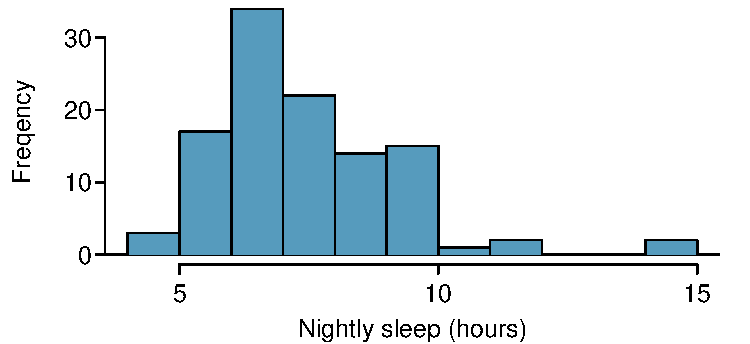
\includegraphics[width=0.7\textwidth]{ch_inference_foundations/figures/histOfSleepForCollegeThatWasCheckingForMoreThan7Hours/histOfSleepForCollegeThatWasCheckingForMoreThan7Hours}
\caption{Distribution of a night of sleep for 110 college students. These data are strongly skewed.\index{skew!example: strong}}
\label{histOfSleepForCollegeThatWasCheckingForMoreThan7Hours}
\end{figure}

Before we can use a normal model for the sample mean or compute the standard error of the sample mean, we must verify conditions. (1)~Because this is a simple random sample from less than 10\% of the student body, the observations are independent. (2)~The sample size in the sleep study is sufficiently large since it is greater than 30. (3)~The data show strong skew in Figure~\ref{histOfSleepForCollegeThatWasCheckingForMoreThan7Hours} and the presence of a couple of outliers. This skew and the outliers are acceptable for a sample size of $n=110$. With these conditions verified, the normal model can be safely applied to $\bar{x}$ and we can reasonably calculate the standard error.

\begin{exercise} \label{findSEOfFirstSleepStudyCheckingGreaterThan7Hours}
In the sleep study, the sample standard deviation was 1.75 hours and the sample size is 110. Calculate the standard error of $\bar{x}$.\footnote{The standard error can be estimated from the sample standard deviation and the sample size: $SE_{\bar{x}} = \frac{s_x}{\sqrt{n}} = \frac{1.75}{\sqrt{110}} = 0.17$.}
\end{exercise}

The hypothesis test for the sleep study will be evaluated using a significance level of $\alpha = 0.05$. We want to consider the data under the scenario that the null hypothesis is true. In this case, the sample mean is from a distribution that is nearly normal and has mean 7 and standard deviation of about $SE_{\bar{x}} = 0.17$. Such a distribution is shown in Figure~\ref{pValueOneSidedSleepStudy}.

\begin{figure}[hht]
   \centering
   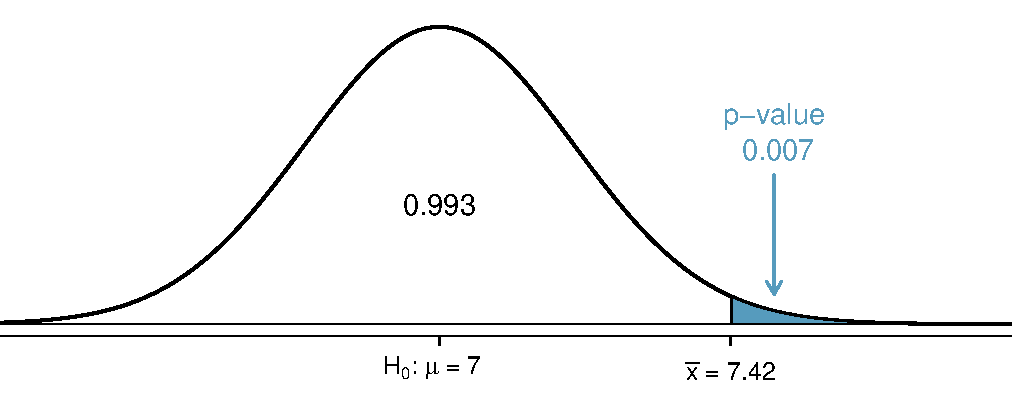
\includegraphics[width=0.83\textwidth]{ch_inference_foundations/figures/pValueOneSidedSleepStudy/pValueOneSidedSleepStudy}
   \caption{If the null hypothesis is true, then the sample mean $\bar{x}$ came from this nearly normal distribution. The right tail describes the probability of observing such a large sample mean if the null hypothesis is true.}
   \label{pValueOneSidedSleepStudy}
\end{figure}

The shaded tail in Figure~\ref{pValueOneSidedSleepStudy} represents the chance of observing such a large mean, conditional on the null hypothesis being true. That is, the shaded tail represents the \mbox{p-value}. We shade all means larger than our sample mean, $\bar{x} = 7.42$, because they are more favorable to the alternative hypothesis than the observed mean.

We compute the p-value by finding the tail area of this normal distribution, which we learned to do in Section~\ref{normalDist}. First compute the Z-score of the sample mean, $\bar{x} = 7.42$:
\begin{eqnarray*}
Z = \frac{\bar{x} - \text{null value}}{SE_{\bar{x}}} = \frac{7.42 - 7}{0.17} = 2.47
\end{eqnarray*}
Using the normal probability table, the lower unshaded area is found to be 0.993. Thus the shaded area is $1-0.993 = 0.007$. {\em If the null hypothesis is true, the probability of observing a sample mean at least as large as 7.42 hours for a sample of 110 students is only 0.007.}\index{p-value!interpretation example} That is, if the null hypothesis is true, we would not often see such a large mean.

We evaluate the hypotheses by comparing the p-value to the significance level. Because the p-value is less than the significance level (p-value $=0.007 < 0.05=\alpha$), we reject the null hypothesis. What we observed is so unusual with respect to the null hypothesis that it casts serious doubt on $H_0$ and provides strong evidence favoring $H_A$.

\begin{termBox}{\tBoxTitle{p-value as a tool in hypothesis testing}
The smaller the p-value, the stronger the data favor $H_A$ over $H_0$. A small p-value (usually $<0.05$) corresponds to sufficient evidence to reject $H_0$ in favor of $H_A$.}
\index{hypothesis testing!p-value|)}
\end{termBox}

\begin{tipBox}{\tipBoxTitle{It is useful to first draw a picture to find the p-value}
It is useful to draw a picture of the distribution of $\bar{x}$ as though $H_0$ was true (i.e.~$\mu$~equals the null value), and shade the region (or regions) of sample means that are at least as favorable to the alternative hypothesis. These shaded regions represent the p-value.}
\end{tipBox}

The ideas below review the process of evaluating hypothesis tests with p-values:
\begin{itemize}
\setlength{\itemsep}{0mm}
\item The null hypothesis represents a skeptic's position or a position of no difference. We reject this position only if the evidence strongly favors $H_A$.
\item A small p-value means that if the null hypothesis is true, there is a low probability of seeing a point estimate at least as extreme as the one we saw. We interpret this as strong evidence in favor of the alternative.
\item We reject the null hypothesis if the p-value is smaller than the significance level, $\alpha$, which is usually 0.05. Otherwise, we fail to reject $H_0$.
\item We should always state the conclusion of the hypothesis test in plain language so non-statisticians can also understand the results.
\end{itemize}

The p-value is constructed in such a way that we can directly compare it to the significance level ($\alpha$) to determine whether or not to reject $H_0$. This method ensures that the Type~1 Error rate does not exceed the significance level standard. 

\begin{figure}[ht]
   \centering
   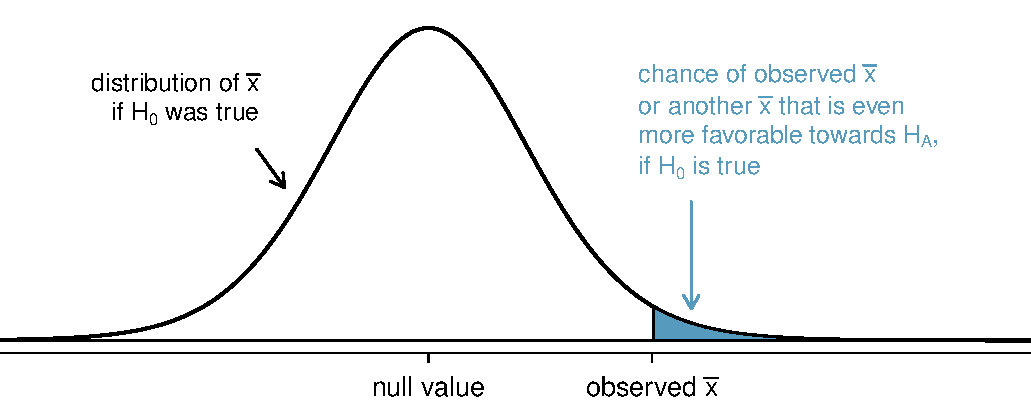
\includegraphics[width=0.9\textwidth]{ch_inference_foundations/figures/pValueOneSidedSleepStudyExplained/pValueOneSidedSleepStudyExplained}
   \caption{To identify the p-value, the distribution of the sample mean is considered as if the null hypothesis was true. Then the p-value is defined and computed as the probability of the observed $\bar{x}$ or an $\bar{x}$ even more favorable to $H_A$ under this distribution.}
   \label{pValueOneSidedSleepStudyExplained}
\end{figure}

\begin{exercise}
If the null hypothesis is true, how often should the p-value be less than 0.05?\footnote{About 5\% of the time. If the null hypothesis is true, then the data only has a 5\% chance of being in the 5\% of data most favorable to $H_A$.}
\index{data!school sleep|)}
\end{exercise}

\begin{exercise}
Suppose we had used a significance level of 0.01 in the sleep study. Would the evidence have been strong enough to reject the null hypothesis? (The p-value was 0.007.) What if the significance level was $\alpha = 0.001$? \footnote{We reject the null hypothesis whenever $p$-$value < \alpha$. Thus, we would still reject the null hypothesis if $\alpha = 0.01$ but not if the significance level had been $\alpha = 0.001$.}
\end{exercise}

\begin{exercise} \label{ebayAmazonOneSidedTestExercise}
\index{data!mario\_kart|(}
Ebay might be interested in showing that buyers on its site tend to pay less than they would for the corresponding new item on Amazon. We'll research this topic for one particular product: a video game called \emph{Mario Kart} for the Nintendo Wii. During early October 2009, Amazon sold this game for \$46.99. Set up an appropriate (one-sided!) hypothesis test to check the claim that Ebay buyers pay less during auctions at this same time.\footnote{The skeptic would say the average is the same on Ebay, and we are interested in showing the average price is lower.
\begin{itemize}
\setlength{\itemsep}{0mm}
\item[$H_0$:] The average auction price on Ebay is equal to (or more than) the price on Amazon. We write only the equality in the statistical notation: $\mu_{ebay} = 46.99$.
\item[$H_A$:] The average price on Ebay is less than the price on Amazon, $\mu_{ebay} < 46.99$.
\end{itemize}}
\end{exercise}


\begin{exercise} \label
{exerciseFor52EbayAuctionsToExamineMarioKartLessExpensiveThanAmazonConditions}
During early October 2009, 52 Ebay auctions were recorded for \emph{Mario Kart}.\footnote{These data were collected by OpenIntro staff.} The total prices for the auctions are presented using a histogram in Figure~\ref{ebayMarioKartAuctionPriceHistogramFor3ConditionsExercise}, and we may like to apply the normal model to the sample mean. Check the three conditions required for applying the normal model: (1)~independence, (2)~at~least 30 observations, and (3)~the data are not strongly skewed.\footnote{(1) The independence condition is unclear. \emph{We will make the assumption that the observations are independent, which we should report with any final results.} (2) The sample size is sufficiently large: $n =52 \geq 30$. (3) The data distribution is not strongly skewed; it is approximately symmetric.}
\end{exercise}

\begin{figure}
   \centering
   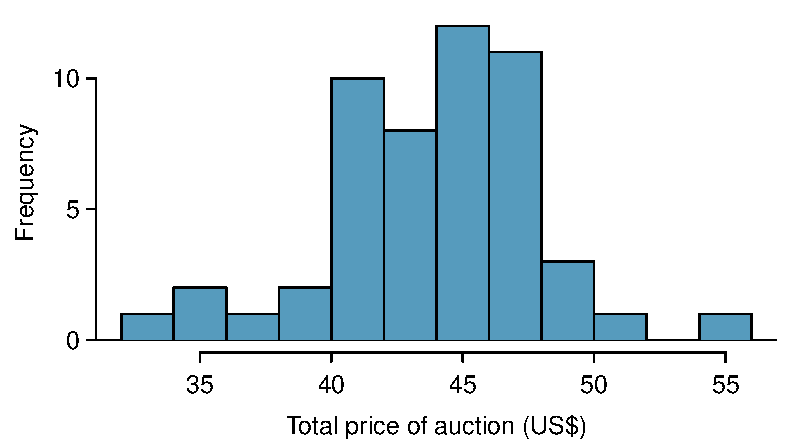
\includegraphics[width=0.77\textwidth]{ch_inference_foundations/figures/ebayMarioKartAuctionPriceHistogramFor3ConditionsExercise/ebayMarioKartAuctionPriceHistogramFor3ConditionsExercise}
   \caption{A histogram of the total auction prices for 52 Ebay auctions.}
   \label{ebayMarioKartAuctionPriceHistogramFor3ConditionsExercise}
\end{figure}

\begin{example}{The average sale price of the 52 Ebay auctions for \emph{Wii Mario Kart} was \$44.17 with a standard deviation of \$4.15. Does this provide sufficient evidence to reject the null hypothesis in Guided Practice~\ref{ebayAmazonOneSidedTestExercise}? Use a significance level of $\alpha = 0.01$.}
The hypotheses were set up and the conditions were checked in Exercises~\ref{ebayAmazonOneSidedTestExercise} and~\ref{exerciseFor52EbayAuctionsToExamineMarioKartLessExpensiveThanAmazonConditions}. The next step is to find the standard error of the sample mean and produce a sketch to help find the p-value.
\begin{eqnarray*}
SE_{\bar{x}} = s/\sqrt{n} = 4.15/\sqrt{52} = 0.5755
\end{eqnarray*}
\begin{center}
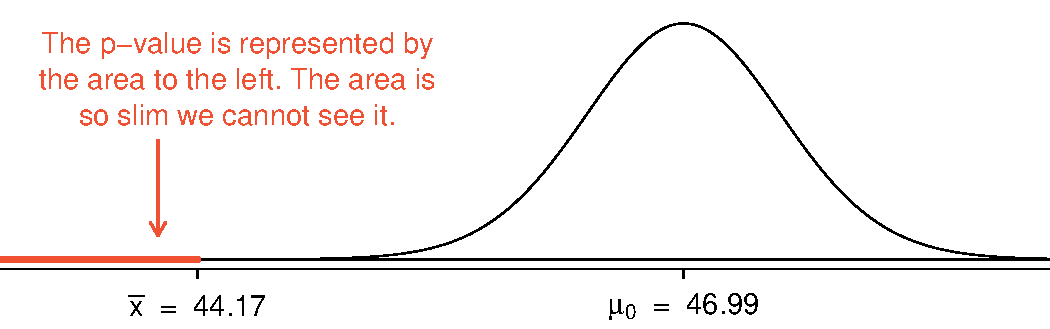
\includegraphics[height=35mm]{ch_inference_foundations/figures/pVForEbayAmazonComparison/pVForEbayAmazonComparison}
\end{center}
Because the alternative hypothesis says we are looking for a smaller mean, we shade the lower tail. We find this shaded area by using the Z-score and normal probability table: $Z = \frac{44.17 - 46.99}{0.5755} = -4.90$, which has area less than 0.0002. The area is so small we cannot really see it on the picture. This lower tail area corresponds to the p-value.

Because the p-value is so small -- specifically, smaller than $\alpha = 0.01$ -- this provides sufficiently strong evidence to reject the null hypothesis in favor of the alternative. The data provide statistically significant evidence that the average price on Ebay is lower than Amazon's asking price.
\index{data!mario\_kart|)}
\end{example}

\begin{termBox}{\tBoxTitle{What's so special about 0.05?}
It's common to use a threshold of 0.05 to determine whether a result is statistically significant, but why is the most common value 0.05? Maybe the standard significance level should be bigger, or maybe it should be smaller. If you're a little puzzled, that probably means you're reading with a critical eye -- good job! We've made a 5-minute task to help clarify \emph{why 0.05}:
\begin{center}
\oiRedirect{textbook-why05}{www.openintro.org/why05}
\end{center}
Sometimes it's also a good idea to deviate from the standard. We'll discuss when to choose a threshold different than 0.05 in Section~\ref{significanceLevel}.\vspace{0.5mm}}
\end{termBox}


\subsection{Two-sided hypothesis testing with p-values}
\label{twoSidedTestsWithPValues}

\index{data!school sleep|(}

We now consider how to compute a p-value for a two-sided test. In one-sided tests, we shade the single tail in the direction of the alternative hypothesis. For example, when the alternative had the form $\mu > 7$, then the p-value was represented by the upper tail (Figure~\ref{pValueOneSidedSleepStudyExplained}). When the alternative was $\mu < 46.99$, the p-value was the lower tail (Guided Practice~\ref{ebayAmazonOneSidedTestExercise}). In a two-sided test, \emph{we shade two tails} since evidence in either direction is favorable to $H_A$.

\begin{exercise} \label{2ndSchSleepHypSetupExercise}
Earlier we talked about a research group investigating whether the students at their school slept longer than 7 hours each night. Let's consider a second group of researchers who want to evaluate whether the students at their college differ from the norm of 7 hours. Write the null and alternative hypotheses for this investigation.\footnote{Because the researchers are interested in any difference, they should use a two-sided setup: $H_0: \mu = 7$, $H_A: \mu \neq 7$.}
\end{exercise}

\begin{example}{The second college randomly samples 122 students and finds a mean of $\bar{x} = 6.83$ hours and a standard deviation of $s=1.8$ hours. Does this provide strong evidence against $H_0$ in Guided Practice~\ref{2ndSchSleepHypSetupExercise}? Use a significance level of $\alpha=0.05$.}
First, we must verify assumptions. (1) A simple random sample of less than 10\% of the student body means the observations are independent. (2) The sample size is 122, which is greater than 30. (3) Based on the earlier distribution and what we already know about college student sleep habits, the sample size will be acceptable.

Next we can compute the standard error ($SE_{\bar{x}} = \frac{s}{\sqrt{n}} = 0.16$) of the estimate and create a picture to represent the p-value, shown in Figure~\ref{2ndSchSleepHTExample}. Both tails are shaded. An estimate of 7.17 or more provides at least as strong of evidence against the null hypothesis and in favor of the alternative as the observed estimate, $\bar{x} = 6.83$.

We can calculate the tail areas by first finding the lower tail corresponding to $\bar{x}$:
\begin{eqnarray*}
Z = \frac{6.83 - 7.00}{0.16} = -1.06 \quad\stackrel{table}{\rightarrow}\quad \text{left tail} = 0.1446
\end{eqnarray*}
Because the normal model is symmetric, the right tail will have the same area as the left tail. The p-value is found as the sum of the two shaded tails:
\begin{eqnarray*}
\text{p-value} = \text{left tail} + \text{right tail} = 2\times(\text{left tail}) = 0.2892
\end{eqnarray*}
This p-value is relatively large (larger than $\alpha=0.05$), so we should not reject $H_0$. That is, if $H_0$ is true, it would not be very unusual to see a sample mean this far from 7 hours simply due to sampling variation. Thus, we do not have sufficient evidence to conclude that the mean is different than 7 hours.

\index{data!school sleep|)}

\begin{figure}
   \centering
   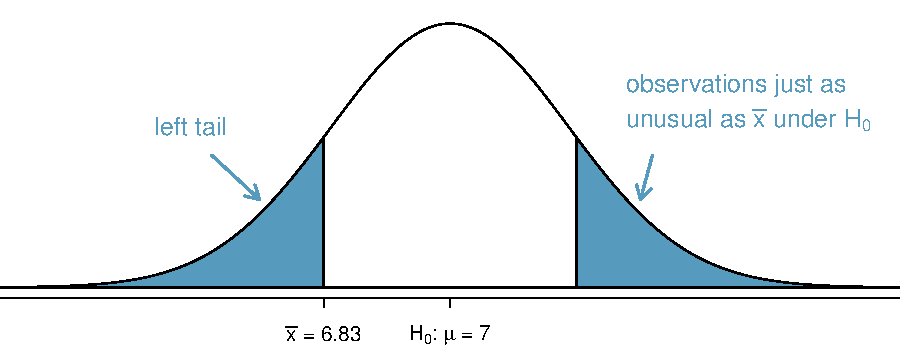
\includegraphics[width=0.9\textwidth]{ch_inference_foundations/figures/2ndSchSleepHTExample/2ndSchSleepHTExample}
   \caption{$H_A$ is two-sided, so \emph{both} tails must be counted for the p-value.}
   \label{2ndSchSleepHTExample}
\end{figure}

\end{example}

\begin{example}{It is never okay to change two-sided tests to one-sided tests after observing the data. In this example we explore the consequences of ignoring this advice. Using $\alpha=0.05$, we show that freely switching from two-sided tests to one-sided tests will cause us to make twice as many Type~1 Errors as intended.} \label{swappingHypAfterDataDoublesType1ErrorRate}
Suppose the sample mean was larger than the null value, $\mu_0$ (e.g. $\mu_0$ would represent~7 if $H_0$:~$\mu = 7$). Then if we can flip to a one-sided test, we would use $H_A$: $\mu > \mu_0$. Now if we obtain any observation with a Z-score greater than 1.65, we would reject $H_0$. If the null hypothesis is true, we incorrectly reject the null hypothesis about 5\% of the time when the sample mean is above the null value, as shown in Figure~\ref{type1ErrorDoublingExampleFigure}.

Suppose the sample mean was smaller than the null value. Then if we change to a one-sided test, we would use $H_A$: $\mu < \mu_0$. If $\bar{x}$ had a Z-score smaller than -1.65, we would reject $H_0$. If the null hypothesis is true, then we would observe such a case about 5\% of the time.

By examining these two scenarios, we can determine that we will make a Type~1 Error $5\%+5\%=10\%$ of the time if we are allowed to swap to the ``best'' one-sided test for the data. This is twice the error rate we prescribed with our significance level: $\alpha=0.05$ (!).

\begin{figure}
   \centering
   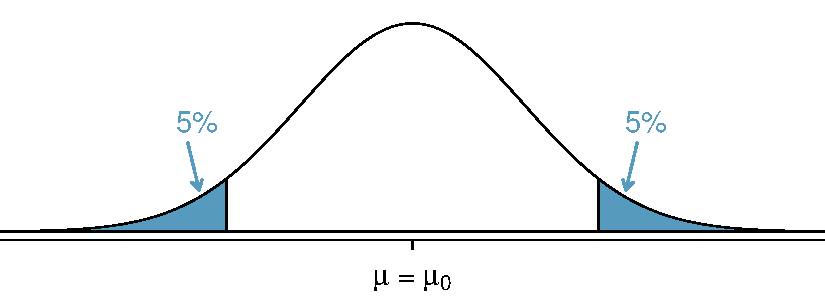
\includegraphics[width=0.7\textwidth]{ch_inference_foundations/figures/type1ErrorDoublingExampleFigure/type1ErrorDoublingExampleFigure}
   \caption{The shaded regions represent areas where we would reject $H_0$ under the bad practices considered in Example~\ref{swappingHypAfterDataDoublesType1ErrorRate} when $\alpha = 0.05$.}
   \label{type1ErrorDoublingExampleFigure}
\end{figure}

\end{example}

\begin{caution}{One-sided hypotheses are allowed only \emph{before} seeing data}
{After observing data, it is tempting to turn a two-sided test into a one-sided test. Avoid this temptation. Hypotheses must be set up \emph{before} observing the data. If~they are not, the test should be two-sided.}
\end{caution}


\subsection{Choosing a significance level}
\label{significanceLevel}

\index{hypothesis testing!significance level|(}
\index{significance level|(}

Choosing a significance level for a test is important in many contexts, and the traditional level is 0.05. However, it is often helpful to adjust the significance level based on the application. We may select a level that is smaller or larger than 0.05 depending on the consequences of any conclusions reached from the test.

If making a Type~1 Error is dangerous or especially costly, we should choose a small significance level (e.g. 0.01). Under this scenario we want to be very cautious about rejecting the null hypothesis, so we demand very strong evidence favoring $H_A$ before we would reject $H_0$.

If a Type~2 Error is relatively more dangerous or much more costly than a Type~1 Error, then we should choose a higher significance level (e.g. 0.10). Here we want to be cautious about failing to reject $H_0$ when the null is actually false.

\begin{tipBox}{\tipBoxTitle[]{Significance levels should reflect consequences of errors}
The significance level selected for a test should reflect the consequences associated with Type~1 and Type~2 Errors.}
\end{tipBox}

\begin{example}{A car manufacturer is considering a higher quality but more expensive supplier for window parts in its vehicles. They sample a number of parts from their current supplier and also parts from the new supplier. They decide that if the high quality parts will last more than 12\% longer, it makes financial sense to switch to this more expensive supplier. Is there good reason to modify the significance level in such a hypothesis test?}
The null hypothesis is that the more expensive parts last no more than 12\% longer while the alternative is that they do last more than 12\% longer. This decision is just one of the many regular factors that have a marginal impact on the car and company. A significance level of 0.05 seems reasonable since neither a Type~1 or Type~2 Error should be dangerous or (relatively) much more expensive.
\end{example}

\begin{example}{The same car manufacturer is considering a slightly more expensive supplier for parts related to safety, not windows. If the durability of these safety components is shown to be better than the current supplier, they will switch manufacturers. Is there good reason to modify the significance level in such an evaluation?}
The null hypothesis would be that the suppliers' parts are equally reliable. Because safety is involved, the car company should be eager to switch to the slightly more expensive manufacturer (reject $H_0$) even if the evidence of increased safety is only moderately strong. A slightly larger significance level, such as $\alpha=0.10$, might be appropriate.
\end{example}

\begin{exercise}
A part inside of a machine is very expensive to replace. However, the machine usually functions properly even if this part is broken, so the part is replaced only if we are extremely certain it is broken based on a series of measurements. Identify appropriate hypotheses for this test (in plain language) and suggest an appropriate significance level.\footnote{Here the null hypothesis is that the part is not broken, and the alternative is that it is broken. If we don't have sufficient evidence to reject $H_0$, we would not replace the part. It sounds like failing to fix the part if it is broken ($H_0$ false, $H_A$ true) is not very problematic, and replacing the part is expensive. Thus, we should require very strong evidence against $H_0$ before we replace the part. Choose a small significance level, such as $\alpha=0.01$.}
\end{exercise}\textC{\vspace{-3mm}}

\index{significance level|)}
\index{hypothesis testing!significance level|)}
\index{hypothesis testing|)}




%__________________
\section[Examining the Central Limit Theorem]{Examining the Central Limit Theorem \sectionvideohref{youtube-lsCc_pS3O28&list=PLkIselvEzpM7Pjo94m1e7J5jkIZkbQAl4}}
\label{cltSection}

\index{Central Limit Theorem|(}

The normal model for the sample mean tends to be very good when the sample consists of at least 30 independent observations and the population data are not strongly skewed. The Central Limit Theorem provides the theory that allows us to make this assumption.

\begin{termBox}{\tBoxTitle{Central Limit Theorem, informal definition}
The distribution of $\bar{x}$ is approximately normal. The approximation can be poor if the sample size is small, but it improves with larger sample sizes.}
\end{termBox}

The Central Limit Theorem states that when the sample size is small, the normal approximation may not be very good. However, as the sample size becomes large, the normal approximation improves. We will investigate three cases to see roughly when the approximation is reasonable.

We consider three data sets: one from a \emph{uniform} distribution, one from an \emph{exponential} distribution, and the other from a \emph{log-normal} distribution. These distributions are shown in the top panels of Figure~\ref{cltSimulations}. The uniform distribution is symmetric, the exponential distribution may be considered as having moderate skew since its right tail is relatively short (few outliers), and the log-normal distribution is strongly skewed and will tend to produce more apparent outliers.\index{skew!example: moderate}\index{skew!example: strong}

\begin{figure}
   \centering
   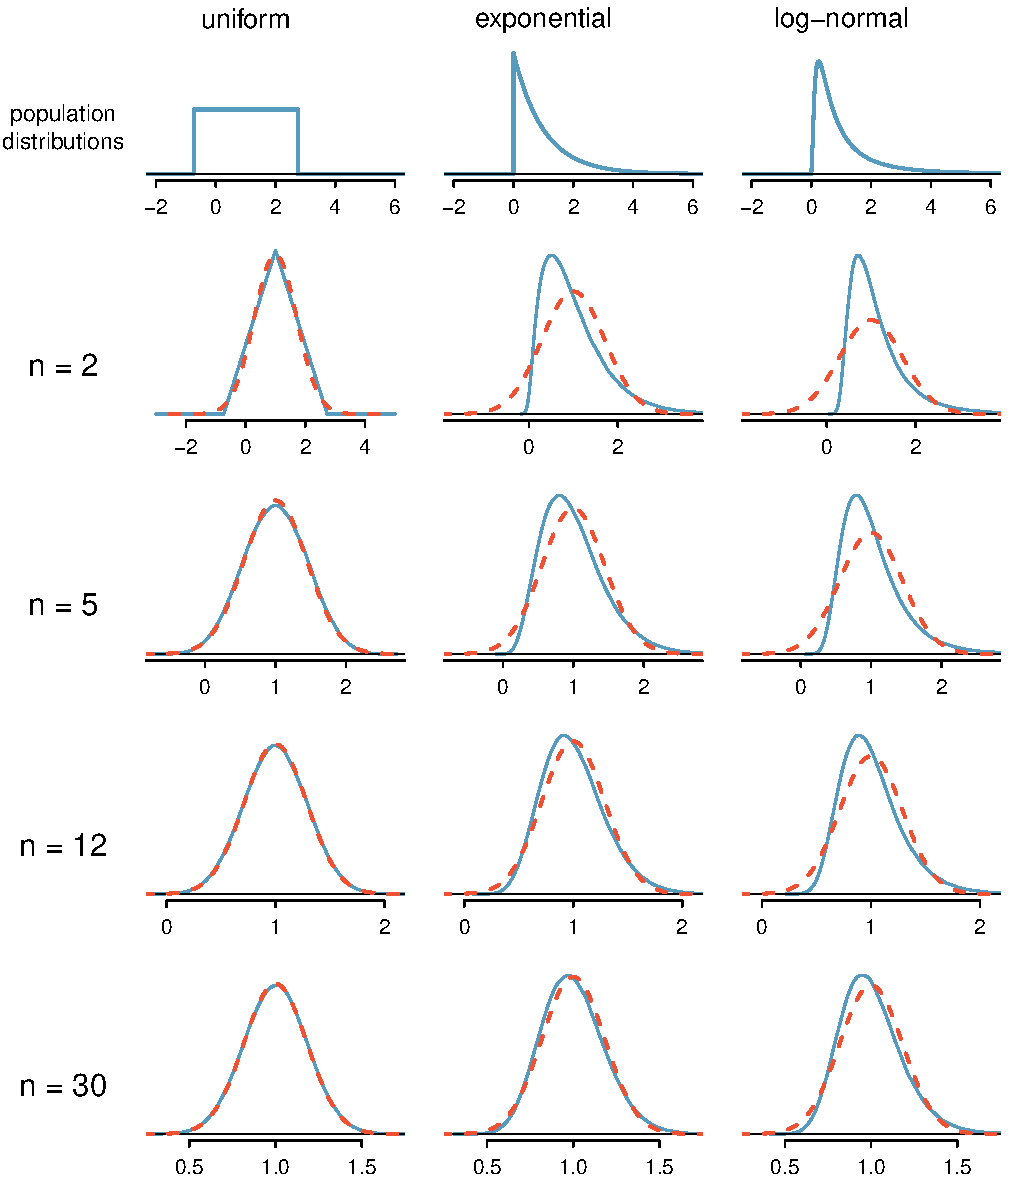
\includegraphics[width=\textwidth]{ch_inference_foundations/figures/cltSimulations/cltSimulations}
   \caption{Sampling distributions for the mean at different sample sizes and for three different distributions. The dashed red lines show normal distributions.}
   \label{cltSimulations}
\end{figure}

The left panel in the $n=2$ row represents the sampling distribution of $\bar{x}$ if it is the sample mean of two observations from the uniform distribution shown. The dashed line represents the closest approximation of the normal distribution. Similarly, the center and right panels of the $n=2$ row represent the respective distributions of $\bar{x}$ for data from exponential and log-normal distributions.

\begin{exercise}
Examine the distributions in each row of Figure~\ref{cltSimulations}. What do you notice about the normal approximation for each sampling distribution as the sample size becomes larger?\footnote{The normal approximation becomes better as larger samples are used.}
\end{exercise}

\begin{example}{Would the normal approximation be good in all applications where the sample size is at least 30?}
Not necessarily. For example, the normal approximation for the log-normal example is questionable for a sample size of 30. Generally, the more skewed a population distribution or the more common the frequency of outliers, the larger the sample required to guarantee the distribution of the sample mean is nearly normal.
\end{example}

\begin{tipBox}{\tipBoxTitle{With larger $n$, the sampling distribution of $\bar{x}$ becomes more normal}
As the sample size increases, the normal model for $\bar{x}$ becomes more reasonable. We can also relax our condition on skew when the sample size is very large.}
\end{tipBox}

We discussed in Section~\ref{seOfTheMean} that the sample standard deviation, $s$, could be used as a substitute of the population standard deviation, $\sigma$, when computing the standard error. This estimate tends to be reasonable when $n\geq30$. We will encounter alternative distributions for smaller sample sizes in Chapters~\ref{inferenceForNumericalData} and~\ref{inferenceForCategoricalData}.

\begin{example}{Figure~\ref{pokerProfitsCanApplyNormalToSampMean} shows a histogram of 50 observations. These represent winnings and losses from 50 consecutive days of a professional poker player. Can the normal approximation be applied to the sample mean, 90.69?}
We should consider each of the required conditions.
\begin{itemize}
\setlength{\itemsep}{0mm}
\item[(1)] These are referred to as \term{time series data}, because the data arrived in a particular sequence. If the player wins on one day, it may influence how she plays the next. To make the assumption of independence we should perform careful checks on such data. While the supporting analysis is not shown, no evidence was found to indicate the observations are not independent.
\item[(2)] The sample size is 50, satisfying the sample size condition.
\item[(3)] There are two outliers, one very extreme, which suggests the data are very strongly skewed or very distant outliers may be common for this type of data. Outliers can play an important role and affect the distribution of the sample mean and the estimate of the standard error.
\end{itemize}
Since we should be skeptical of the independence of observations and the very extreme upper outlier poses a challenge, we should not use the normal model for the sample mean of these 50 observations. If we can obtain a much larger sample, perhaps several hundred observations, then the concerns about skew and outliers would no longer apply.
\end{example}

\begin{figure}[ht]
   \centering
   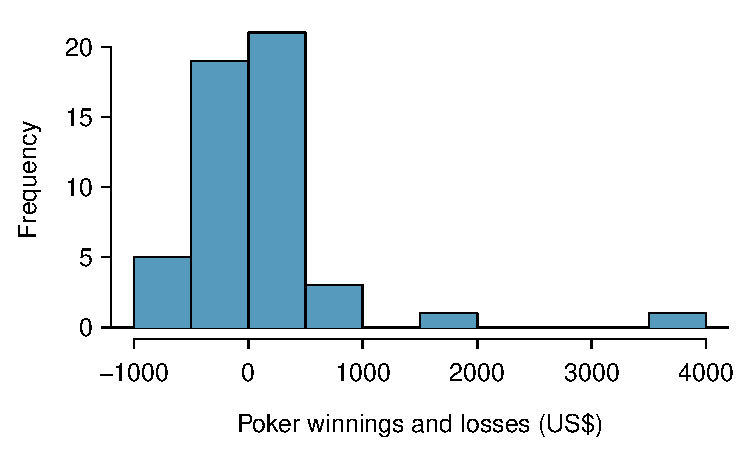
\includegraphics[height=58mm]{ch_inference_foundations/figures/pokerProfitsCanApplyNormalToSampMean/pokerProfitsCanApplyNormalToSampMean}
   \caption{Sample distribution of poker winnings. These data include some very clear outliers. These are problematic when considering the normality of the sample mean. For example, outliers are often an indicator of very strong skew\index{skew!example: very strong}.}
   \label{pokerProfitsCanApplyNormalToSampMean}
\end{figure}

\begin{caution}
{Examine data structure when considering independence}
{Some data sets are collected in such a way that they have a natural underlying structure between observations, e.g. when observations occur consecutively. Be especially cautious about independence assumptions regarding such data sets.}
\end{caution}

\begin{caution}{Watch out for strong skew and outliers}
{Strong skew is often identified by the presence of clear outliers. If a data set has prominent outliers, or such observations are somewhat common for the type of data under study, then it is useful to collect a sample with many more than 30 observations if the normal model will be used for $\bar{x}$.}
\index{Central Limit Theorem|)}
\end{caution}

You won't be a pro at assessing skew by the end of this book, so just use your best judgement and continue learning. As you develop your statistics skills and encounter tough situations, also consider learning about better ways to analyze skewed data, such as the studentized bootstrap (bootstrap-t), or consult a more experienced statistician.

\index{skew!strongly skewed guideline}


%__________________
\section[Inference for other estimators]{Inference for other estimators \sectionvideohref{youtube-PUMBNtVKr_g&list=PLkIselvEzpM7Pjo94m1e7J5jkIZkbQAl4}}
\label{aFrameworkForInference}

The sample mean is not the only point estimate for which the sampling distribution is nearly normal. For example, the sampling distribution of sample proportions closely resembles the normal distribution when the sample size is sufficiently large. In this section, we introduce a number of examples where the normal approximation is reasonable for the point estimate. Chapters~\ref{inferenceForNumericalData} and~\ref{inferenceForCategoricalData} will revisit each of the point estimates you see in this section along with some other new statistics.

We make another important assumption about each point estimate encountered in this section: the estimate is unbiased. A point estimate is \term{unbiased} if the sampling distribution of the estimate is centered at the parameter it estimates. That is, an unbiased estimate does not naturally over or underestimate the parameter. Rather, it tends to provide a ``good'' estimate. The sample mean is an example of an unbiased point estimate, as are each of the examples we introduce in this section.

Finally, we will discuss the general case where a point estimate may follow some distribution other than the normal distribution. We also provide guidance about how to handle scenarios where the statistical techniques you are familiar with are insufficient for the problem at hand.


\subsection{Confidence intervals for nearly normal point estimates}

\index{confidence interval!using normal model|(}

In Section~\ref{confidenceIntervals}, we used the point estimate $\bar{x}$ with a standard error $SE_{\bar{x}}$ to create a 95\% confidence interval for the population mean:
\begin{align}
\bar{x}\ \pm\ 1.96 \times SE_{\bar{x}}
\label{95PercCIForMeanInGeneralizingSection}
\end{align}
We constructed this interval by noting that the sample mean is within 1.96 standard errors of the actual mean about 95\% of the time. This same logic generalizes to any unbiased point estimate that is nearly normal. We may also generalize the confidence level by using a place-holder $z^{\star}$.

\begin{termBox}{\tBoxTitle{General confidence interval for the normal sampling distribution case}\label{generalConfidenceIntervalTermBox}%
A confidence interval based on an unbiased and nearly normal point estimate is
\begin{eqnarray}
\text{point estimate}\ \pm\ z^{\star}SE
\label{95PercGeneralCIInGeneralizingSection}
\end{eqnarray}
where $z^{\star}$ is selected to correspond to the confidence level, and $SE$ represents the standard error. The value $z^{\star}SE$ is called the \emph{margin of error}\index{margin of error}.}
\end{termBox}

Generally the standard error for a point estimate is estimated from the data and computed using a formula. For example, the standard error for the sample mean is
\begin{eqnarray*}
SE_{\bar{x}} = \frac{s}{\sqrt{n}}
\end{eqnarray*}
In this section, we provide the computed standard error for each example and exercise without detailing where the values came from. In future chapters, you will learn to fill in these and other details for each situation.

\begin{example}{In Guided Practice~\vref{peOfDiffActiveBetweenGender}, we computed a point estimate for the difference in the average days active per week between male and female students: $\bar{x}_{female}-\bar{x}_{male}=1.1$~days. This point estimate is associated with a nearly normal distribution with standard error $SE = 0.5$~days. What is a reasonable 95\% confidence interval for the difference in average days active per week?}
\label{ciForDiffOfPhysActiveBetweenGenders}
The normal approximation is said to be valid, so we apply Equation~\eqref{95PercGeneralCIInGeneralizingSection}:
\begin{eqnarray*}
\text{point estimate}\ \pm\ z^{\star} SE
	\quad\rightarrow\quad 1.1\ \pm\ 1.96\times 0.5
	\quad\rightarrow\quad (0.12, 2.08)
\end{eqnarray*}
We are 95\% confident that the male students, on average, were physically active 0.12 to 2.08 days more than female students in YRBSS each week. That is, the actual average difference is plausibly between 0.12 and 2.08 days per week with 95\% confidence.
\end{example}
%library(openintro); library(xtable); data(yrbss); data(yrbss.samp); (x <- by(yrbss.samp$physically_active_7d, yrbss.samp$gender, mean)); diff(x); s <- by(yrbss.samp$physically_active_7d, yrbss.samp$gender, sd); n <- by(yrbss.samp$physically_active_7d, yrbss.samp$gender, length); sqrt(sum(s^2/n))


\begin{example}{Does Example~\ref{ciForDiffOfPhysActiveBetweenGenders} guarantee that if a male and female student are selected at random from YRBSS, the male student would be active 0.12 to 2.08 days more than the female student?}
Our confidence interval says absolutely nothing about individual observations. It {only} makes a statement about a plausible range of values for the \emph{average} difference between all male and female students who participated in YRBSS.
\end{example}

\begin{exercise} \label{findZFor99PercConfLevelInFrameworkForInf}
What $z^{\star}$ would be appropriate for a 99\% confidence level? For help, see Figure~\vref{choosingZForCI}.\footnote{We seek $z^{\star}$ such that 99\% of the area under the normal curve will be between the Z-scores -$z^{\star}$ and $z^{\star}$. Because the remaining 1\% is found in the tails, each tail has area 0.5\%, and we can identify -$z^{\star}$ by looking up 0.0050 in the normal probability table: $z^{\star} = 2.58$. See also Figure~\vref{choosingZForCI}.}
\end{exercise}

\textC{\newpage}

\begin{exercise}
The proportion of students who are male in the \data{yrbss\_samp} sample is $\hat{p} = 0.48$. This sample meets certain conditions that ensure $\hat{p}$ will be nearly normal, and the standard error of the estimate is $SE_{\hat{p}} = 0.05$. Create a 90\% confidence interval for the proportion of students in the 2013 YRBSS survey who are male.\footnote{We use $z^{\star}=1.65$ (see Guided Practice~~\vref{find90CIForYrbssAgeExercise}), and apply the general confidence interval formula:
\begin{eqnarray*}
\hat{p}\ \pm\ z^{\star}SE_{\hat{p}}
	\quad\to\quad 0.48\ \pm\ 1.65\times 0.05
	\quad\to\quad (0.3975, 0.5625)
\end{eqnarray*}
Thus, we are 90\% confident that between 40\% and 56\% of the YRBSS students were male.}
\index{confidence interval!using normal model|)}
\end{exercise}


\subsection{Hypothesis testing for nearly normal point estimates}
\index{hypothesis testing!using normal model|(}

Just as the confidence interval method works with many other point estimates, we can generalize our hypothesis testing methods to new point estimates. Here we only consider the p-value approach, introduced in Section~\ref{pValue}, since it is the most commonly used technique and also extends to non-normal cases.

\begin{termBox}{\tBoxTitle[]{Hypothesis testing using the normal model}
\begin{enumerate}
\setlength{\itemsep}{0mm}
\item First write the hypotheses in plain language, then set them up in mathematical notation.
\item Identify an appropriate point estimate of the parameter of interest.
\item Verify conditions to ensure the standard error estimate is reasonable and the point estimate is nearly normal and unbiased.
\item Compute the standard error. Draw a picture depicting the distribution of the estimate under the idea that $H_0$ is true. Shade areas representing the p-value.
\item Using the picture and normal model, compute the \emph{test statistic} (Z-score) and identify the p-value to evaluate the hypotheses. Write a conclusion in plain language.
\end{enumerate}}
\end{termBox}

\begin{exercise} \label{fdaHypSetupForSulph}
A drug called sulphinpyrazone was under consideration for use in reducing the death rate in heart attack patients. To determine whether the drug was effective, a set of 1,475 patients were recruited into an experiment and randomly split into two groups: a control group that received a placebo and a treatment group that received the new drug. What would be an appropriate null hypothesis? And the alternative?\footnote{The skeptic's perspective is that the drug does not work at reducing deaths in heart attack patients ($H_0$), while the alternative is that the drug does work ($H_A$).}
\end{exercise}

\textC{\newpage}

We can formalize the hypotheses from Guided Practice~\ref{fdaHypSetupForSulph} by letting $p_{control}$ and $p_{treatment}$ represent the proportion of patients who died in the control and treatment groups, respectively. Then the hypotheses can be written as
\begin{eqnarray*}
&&H_0: p_{control} = p_{treatment} \quad\text{(the drug doesn't work)} \quad \\
&&H_A: p_{control} > p_{treatment} \quad\text{(the drug works)}
\end{eqnarray*}
or equivalently,
\begin{eqnarray*}
&&H_0: p_{control} - p_{treatment} = 0 \quad\text{(the drug doesn't work)} \quad \\
&&H_A: p_{control} - p_{treatment} > 0 \quad\text{(the drug works)}
\end{eqnarray*}
Strong evidence against the null hypothesis and in favor of the alternative would correspond to an observed difference in death rates,
\begin{eqnarray*}
\text{point estimate} = \hat{p}_{control} - \hat{p}_{treatment}
\end{eqnarray*}
being larger than we would expect from chance alone. This difference in sample proportions represents a point estimate that is useful in evaluating the hypotheses. 

\begin{example}{We want to evaluate the hypothesis setup from Exericse~\ref{fdaHypSetupForSulph} using data from the actual study.\footnote{Anturane Reinfarction Trial Research Group. 1980. Sulfinpyrazone in the prevention of sudden death after myocardial infarction. New England Journal of Medicine 302(5):250-256.} In the control group, 60 of 742 patients died. In the treatment group, 41 of 733 patients died. The sample difference in death rates can be summarized as
\begin{eqnarray*}
\text{point estimate} = \hat{p}_{control} - \hat{p}_{treatment} = \frac{60}{742} - \frac{41}{733} = 0.025
\end{eqnarray*}
This point estimate is nearly normal and is an unbiased estimate of the actual difference in death rates. The standard error of this sample difference is $SE = 0.013$. Evaluate the hypothesis test at a 5\% significance level: $\alpha=0.05$.}
We would like to identify the p-value to evaluate the hypotheses. If the null hypothesis is true, then the point estimate would have come from a nearly normal distribution, like the one shown in Figure~\ref{sulphStudyFindPValueUsingNormalApprox}. The distribution is centered at zero since $p_{control}-p_{treatment}=0$ under the null hypothesis. Because a large positive difference provides evidence against the null hypothesis and in favor of the alternative, the upper tail has been shaded to represent the p-value. We need not shade the lower tail since this is a one-sided test: an observation in the lower tail does not support the alternative hypothesis.

\begin{figure}[bt]
   \centering
   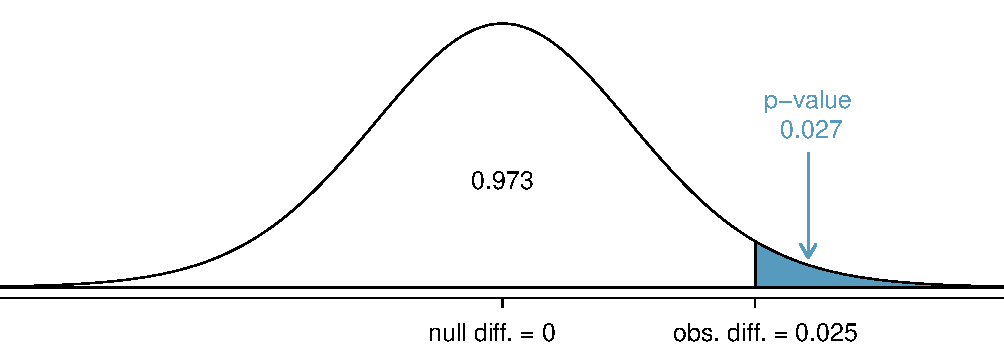
\includegraphics[width=0.88\textwidth]{ch_inference_foundations/figures/sulphStudyFindPValueUsingNormalApprox/sulphStudyFindPValueUsingNormalApprox}
   \caption{The distribution of the sample difference if the null hypothesis is true.}
   \label{sulphStudyFindPValueUsingNormalApprox}
\end{figure}

The p-value can be computed by using the Z-score of the point estimate and the normal probability table.
\begin{eqnarray}
Z = \frac{\text{point estimate} - \text{null value}}{SE_{\text{point estimate}}}
	= \frac{0.025 - 0}{0.013} = 1.92
\label{zScoreOfPointEstimateForSulphinpyrazoneThisIsFirstTestStatReference}
\end{eqnarray}
Examining Z in the normal probability table, we find that the lower unshaded tail is about 0.973. Thus, the upper shaded tail representing the p-value is
\begin{eqnarray*}
\text{p-value} = 1-0.973 = 0.027
\end{eqnarray*}
Because the p-value is less than the significance level ($\alpha=0.05$), we say the null hypothesis is implausible. That is, we reject the null hypothesis in favor of the alternative and conclude that the drug is effective at reducing deaths in heart attack patie
nts.
\end{example}

The Z-score in Equation~(\ref{zScoreOfPointEstimateForSulphinpyrazoneThisIsFirstTestStatReference}) is called a \term{test statistic}. In most hypothesis tests, a test statistic is a particular data summary that is especially useful for computing the p-value and evaluating the hypothesis test. In the case of point estimates that are nearly normal, the test statistic is the Z-score.

\begin{termBox}{\tBoxTitle{Test statistic}
A \emph{test statistic} is a summary statistic that is particularly useful for evaluating a hypothesis test or identifying the p-value. When a point estimate is nearly normal, we use the Z-score of the point estimate as the test statistic. In later chapters we encounter situations where other test statistics are helpful.}
\index{hypothesis testing!using normal model|)}
\end{termBox}


\subsection{Non-normal point estimates}

We may apply the ideas of confidence intervals and hypothesis testing to cases where the point estimate or test statistic is not necessarily normal. There are many reasons why such a situation may arise:
\begin{itemize}
\setlength{\itemsep}{0mm}
\item the sample size is too small for the normal approximation to be valid;
\item the standard error estimate may be poor; or
\item the point estimate tends towards some distribution that is not the normal distribution.
\end{itemize}
For each case where the normal approximation is not valid, our first task is always to understand and characterize the sampling distribution of the point estimate or test statistic. Next, we can apply the general frameworks for confidence intervals and hypothesis testing to these alternative distributions.


\textC{\newpage}


\subsection{When to retreat}
\label{whenToRetreat}

Statistical tools rely on conditions. When the conditions are not met, these tools are unreliable and drawing conclusions from them is treacherous. The conditions for these tools typically come in two forms.
\begin{itemize}
\setlength{\itemsep}{0mm}
\item \textbf{The individual observations must be independent.} A random sample from less than 10\% of the population ensures the observations are independent. In experiments, we generally require that subjects are randomized into groups. If independence fails, then advanced techniques must be used, and in some such cases, inference may not be possible.
\item \textbf{Other conditions focus on sample size and skew.} For example, if the sample size is too small, the skew too strong, or extreme outliers are present, then the normal model for the sample mean will fail.
\end{itemize}
Verification of conditions for statistical tools is always necessary. Whenever conditions are not satisfied for a statistical technique, there are three options. The first is to learn new methods that are appropriate for the data. The second route is to consult a statistician.\footnote{If you work at a university, then there may be campus consulting services to assist you. Alternatively, there are many private consulting firms that are also available for hire.} The third route is to ignore the failure of conditions. This last option effectively invalidates any analysis and may discredit novel and interesting findings.

Finally, we caution that there may be no inference tools helpful when considering data that include unknown biases, such as convenience samples. For this reason, there are books, courses, and researchers devoted to the techniques of sampling and experimental design. See Sections~\ref{overviewOfDataCollectionPrinciples}-\ref{experimentsSection} for basic principles of data collection.


\subsection{Statistical significance versus practical significance}

When the sample size becomes larger, point estimates become more precise and any real differences in the mean and null value become easier to detect and recognize. Even a very small difference would likely be detected if we took a large enough sample. Sometimes researchers will take such large samples that even the slightest difference is detected. While we still say that difference is \term{statistically significant}, it might not be \term{practically significant}.

Statistically significant differences are sometimes so minor that they are not practically relevant. This is especially important to research: if we conduct a study, we want to focus on finding a meaningful result. We don't want to spend lots of money finding results that hold no practical value.

The role of a statistician in conducting a study often includes planning the size of the study. The statistician might first consult experts or scientific literature to learn what would be the smallest meaningful difference from the null value. She also would obtain some reasonable estimate for the standard deviation. With these important pieces of information, she would choose a sufficiently large sample size so that the power for the meaningful difference is perhaps 80\% or 90\%. While larger sample sizes may still be used, she might advise against using them in some cases, especially in sensitive areas of research.